\documentclass[sans,mathserif]{beamer}
%handout,notes=show

%\usepackage{pgfpages}
%\pgfpagesuselayout{8 on 1}[a4paper,border shrink=5mm]

\usetheme{default}
\usepackage{fp}
\usepackage[thicklines]{cancel}
\usepackage{tikz}
\usepackage{multirow}
\usepackage{amsmath}
\usepackage{ifthen}
\usepackage{animate}
\usepackage{setspace}
\usepackage{forloop}
%\usepackage{concmath}
%\usepackage{pxfonts}
%\usepackage{eulervm}
%\usepackage{mathpazo}
%\renewcommand\mathfamilydefault{\rmdefault}

%\usefonttheme{professionalfonts}
%\setmathfont{}
%\setsansfont{Palatino}
\usetikzlibrary{arrows,backgrounds,positioning,fit,chains,shapes,calc,matrix,decorations,decorations.pathreplacing}

%\usepackage{handoutWithNotes}
%\pgfpagesuselayout{4 on 1 with notes}[a4paper,border shrink=5mm]

\setbeamertemplate{navigation symbols}{}

\title{Basics of modern computers}
\author{Dag Sverre Seljebotn}
%\institute{Department of Mathematics \\ University of Oslo}
\date{September 7, 2012}

\newcommand{\V}{\vskip1em}

\setbeamersize{sidebar width left=0cm, sidebar width right=0cm}
\setbeamersize{text margin left=.8cm, text margin right=.8cm}

\defbeamertemplate{note page}{infolines}
{%
  \vskip3em
%  \setstretch{1.8}
  \Large
  \rmfamily
  \insertnote
}
\setbeamertemplate{note page}[infolines]

\renewcommand{\CancelColor}{\color{red}}


\begin{document}


\begin{frame}
  \titlepage
\end{frame}


\begin{frame}

{\small Donald Knuth:}
  \begin{tikzpicture}
    \node[text width=8cm]{
    \begin{quote}
      Programmers waste enormous amounts of time thinking about, or
      worrying about, the speed of noncritical parts of their
      programs, and these attempts at efficiency actually have a
      strong negative impact when debugging and maintenance are
      considered. We should forget about small efficiencies, say about
      97\% of the time: {\bf premature optimization is the root of all
        evil}. Yet we should not pass up our opportunities in that
      critical 3\%.
    \end{quote}
};
    \node at (-5, 0) {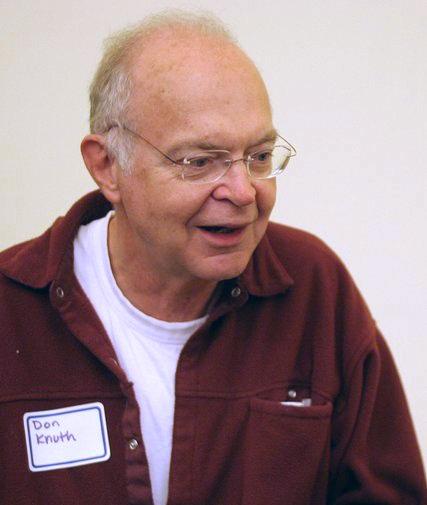
\includegraphics[width=3cm]{knuth.jpg}};
  \end{tikzpicture}
\end{frame}

\begin{frame}{The law of leaky abstractions}
{\small Joel Spolsky:}
  \begin{tikzpicture}
    \node[text width=7cm]{
    \begin{quote}
      {\bf All non-trivial abstractions, to some degree, are leaky.} [...]
      Indeed, the
      abstractions we've created over the years do allow us to deal
      with new orders of complexity in software development that we
      didn't have to deal with ten or fifteen years ago [...].
      Suddenly one day we need to figure
      out a problem where the abstraction leaked, and it takes 2
      weeks.
    \end{quote}
};
    \node at (-5, 0) {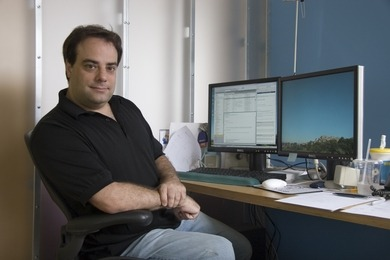
\includegraphics[width=4cm]{spolsky.jpg}};
  \end{tikzpicture}


~

{\small http://www.joelonsoftware.com/articles/LeakyAbstractions.html}
\end{frame}

\begin{frame}{Past decades: Optimism}

``Don't worry, better CPUs and compilers will take care of it''

~

{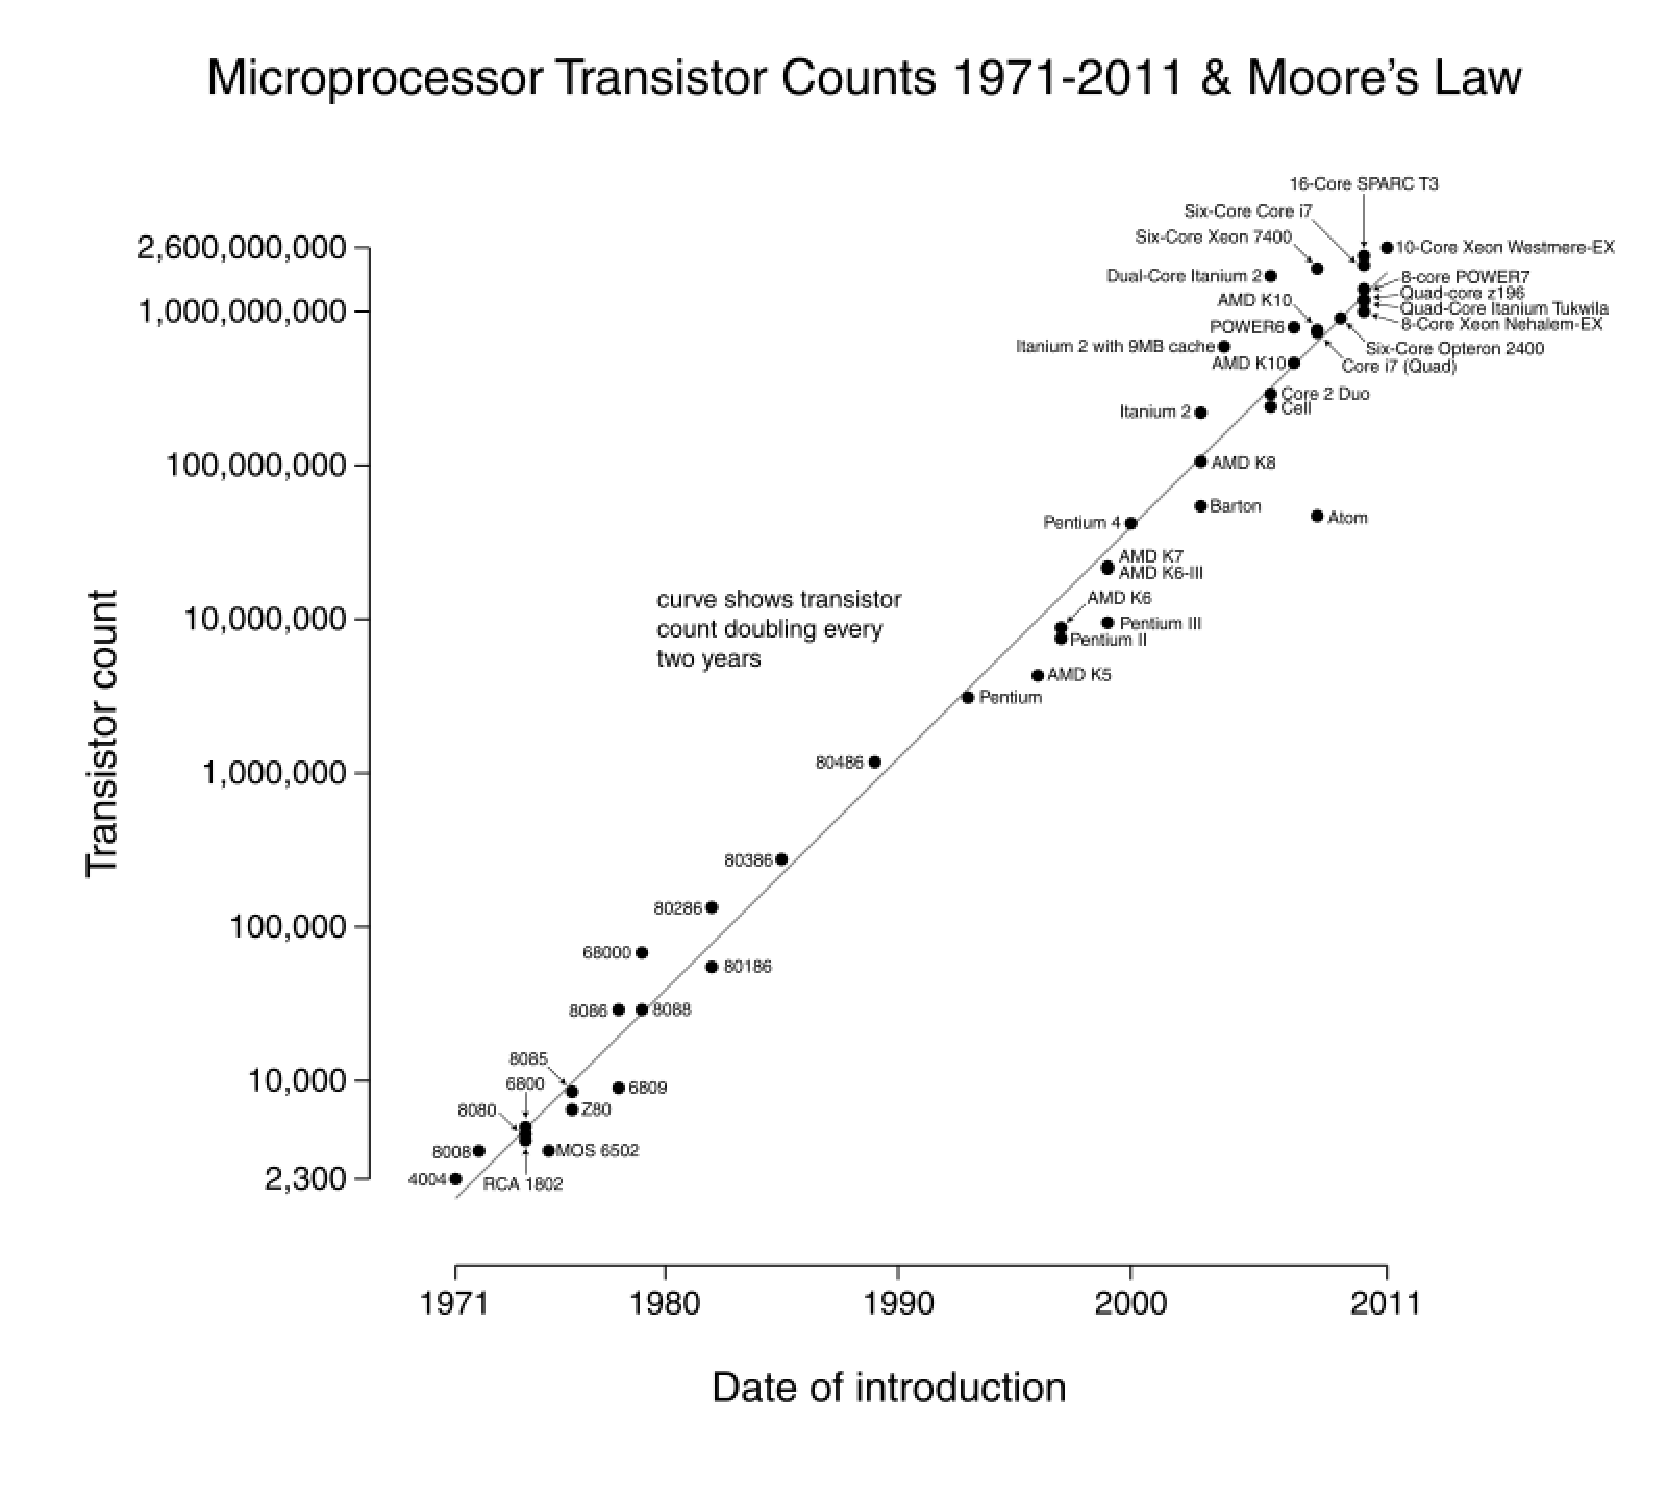
\includegraphics[width=0.8\textwidth]{transistors.pdf}};
\end{frame}

\begin{frame}{The reality}
More complexity; algorithm must be adapted to hardware; compilers no magic bullet

~

  \begin{tikzpicture}
    \uncover<+->{\node at (-2,0) {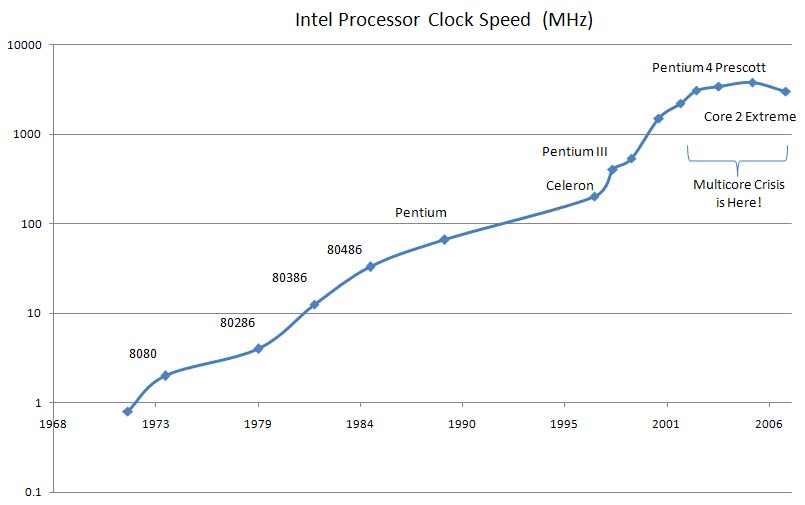
\includegraphics[width=0.8\textwidth]{clockspeeds.jpg}};}
    \uncover<+->{\node at (0,-1) {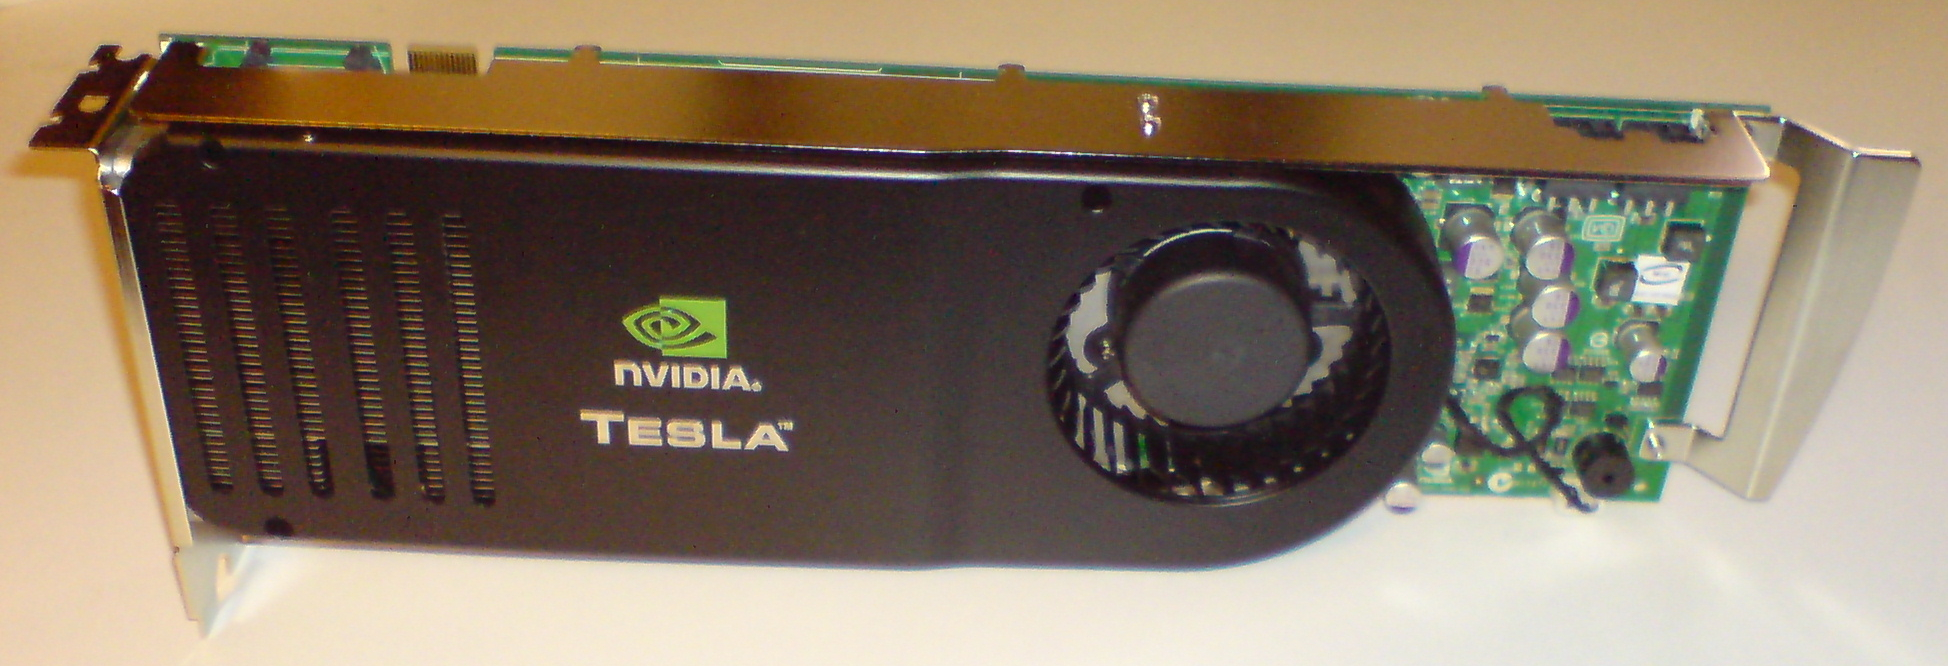
\includegraphics[width=0.9\textwidth]{nvidiatesla.jpg}};}
  \end{tikzpicture}
  
\end{frame}

\begin{frame}

  \begin{center}
    {\Large The basic abstractions for working with computers}
  \end{center}
\end{frame}

% \begin{frame}{Memory, encoding and pointers}
%   \begin{center}
%   von Neumann architecture: CPU $\leftrightarrow$ memory bus $\leftrightarrow$ memory

% ~

%     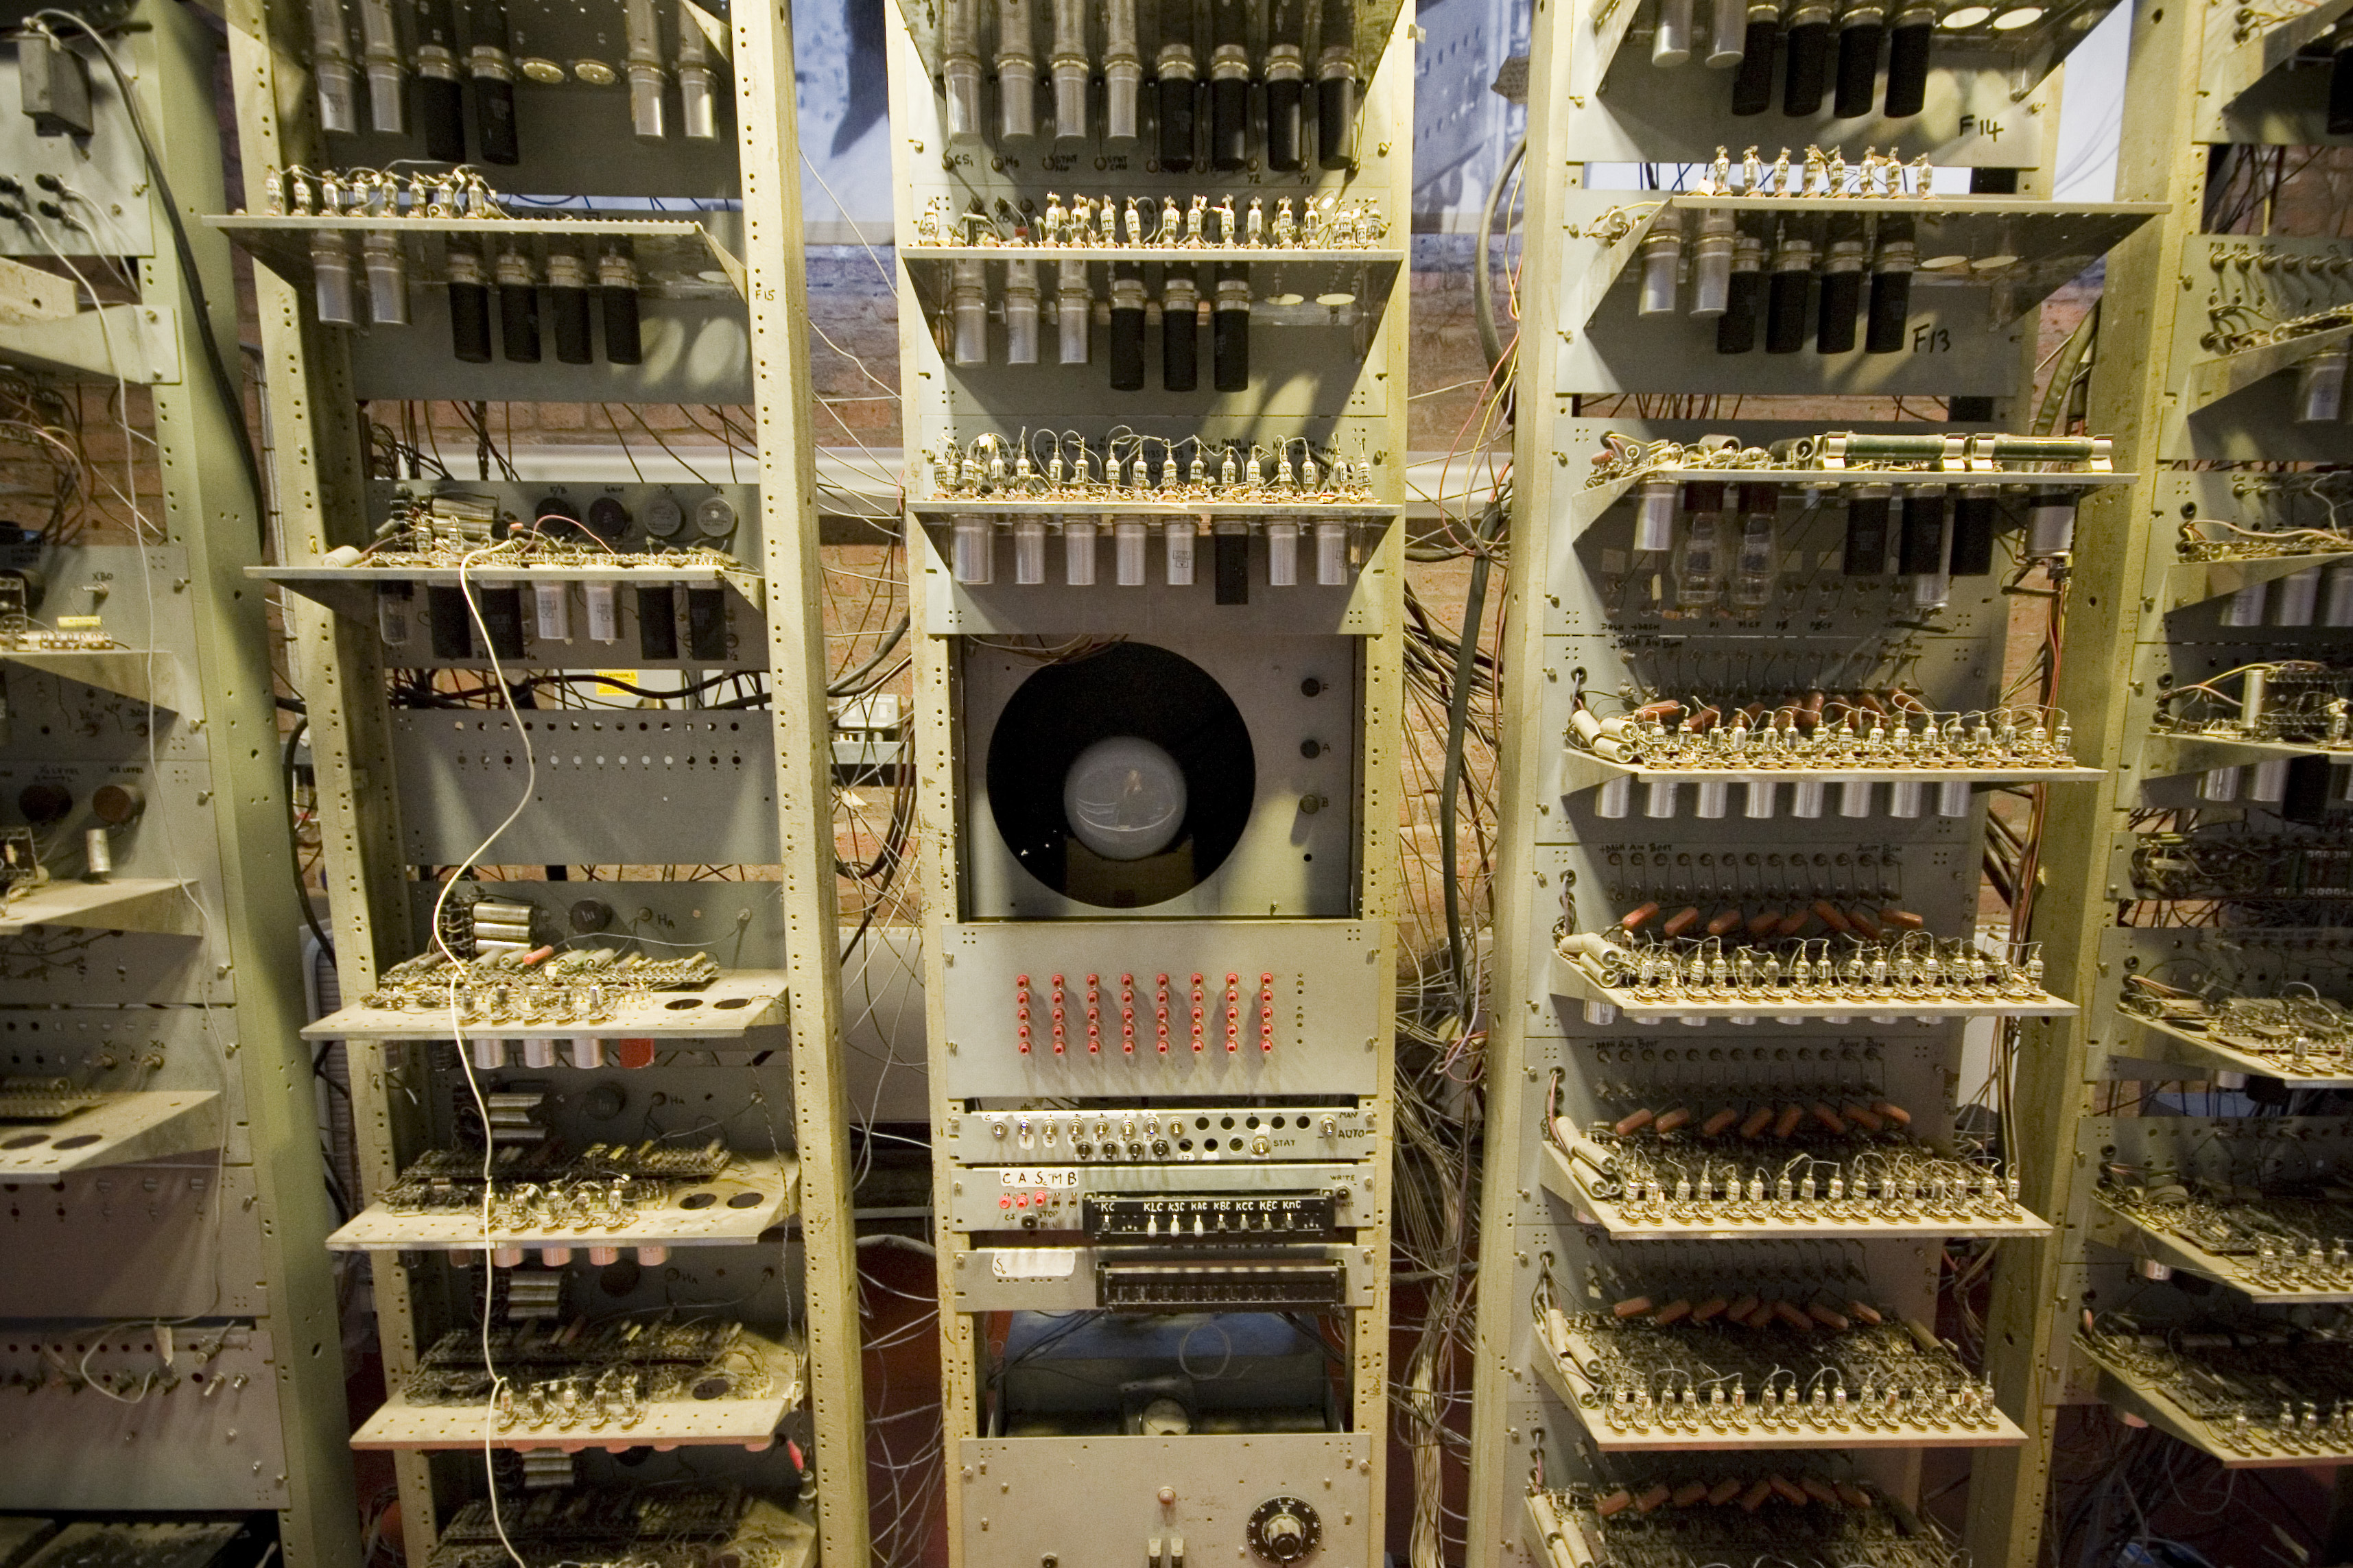
\includegraphics[width=0.7\textwidth]{SSEM.jpg}\\
%     Manchester Small-Scale Experimental Machine, world's first
%     stored-program computer (1948)
%   \end{center}
% \end{frame}

\newcommand{\bs}[3]{{\color{blue}#1} \cdot {#2}^{#3} }
\newcommand{\br}[3]{{\color{red}#1} \cdot {#2}^{#3} }
\begin{frame}{Memory, encoding and pointers}

  Everything (data, program) is encoded in {\em memory bytes},
  which (nowadays) are always 8 bits, allowing $2^8=256$ distinct values.

%124     124    0x7c   |    01111100 
{\small
  \begin{align*}
    124_{10} &= \bs{1}{10}{2} + \bs{2}{10}{1} + \bs{4}{10}{0} \\
    &= \bs{0}{2}{7} + \bs{1}{2}{6} + \bs{1}{2}{5}
              + \bs{1}{2}{4} + 
              \only<1>{\bs{1}{2}{3} + \bs{1}{2}{2} + \bs{0}{2}{1} + \bs{0}{2}{0}}
              \only<2>{\br{1}{2}{3} + \br{1}{2}{2} + \br{0}{2}{1} + \br{0}{2}{0}}
              \\
\uncover<2->{
 &= \bs{7}{16}{1} + \br{12}{16}{0} = \text{\tt 0x{\color{blue}7}{\color{red}c}}}
  \end{align*}
}

  Demo: {\tt binary.c}
\end{frame}

\begin{frame}{Pointers (as seen in C)}
  \begin{tabular}{lll}
    \uncover<+->{{\tt int32\_t x;} & \quad Declare a 4-byte integer ``x'' \\}
    \uncover<+->{{\tt x = 42;} & \quad Memory of ``x'' now contains 42 \\}
    \uncover<+->{{\tt int32\_t *p;} & \quad Declare an 8-byte {\bf pointer to int} ``p'' \\}
    \uncover<+->{{\tt p = \&x;} & \quad Memory of ``p'' now contains 0x00007fffa63cc4b0 \\}
    \uncover<+->{{\tt *p = 10;} & \quad Memory of ``x'' now contains 10}
  \end{tabular}
\end{frame}

\begin{frame}{Pointers and arrays...}
  \begin{tabular}{lll}
    \uncover<+->{{\tt int32\_t *p} & \quad\quad ``x'' is a pointer to integers \\}
    \uncover<+->{{\tt p = malloc(40);} & \quad\quad Allocate space for 10 integers (``array'') \\
     {\tt } & \quad\quad Memory of ``x'' contains 0x00007fffa63cc4b0 \\}
    \uncover<+->{{\tt int32\_t *u;} & \quad\quad  \\}
    \uncover<+->{{\tt u = p + 1;} & \quad\quad Memory of ``u'' contains 0x00007fffa63cc4b4   \\}
    \uncover<+->{{\tt *p = 10;} & \quad\quad Assign first element of array   \\}
    \uncover<+->{{\tt *u = 20;} & \quad\quad Assign second element of array   \\ & \\}

    \uncover<+->{{\tt p[0] = 10;} & \quad\quad Same as {\tt *p = 10} \\ }
    \uncover<+->{{\tt p[1] = 20;} & \quad\quad Same as {\tt *(p + 1) = 20} \\ }
    \uncover<+->{{\tt p[10] = 30;} & \quad\quad Trampling on unallocated memory! \\ }
  \end{tabular}
\end{frame}

\begin{frame}[fragile]{Multi-dimensional arrays}
\begin{verbatim}
int32_t array = malloc(400);
int32_t nrows = 5, ncols = 20;

/* Treat memory in row-major ordering (C-order) */
for (int32_t i = 0; i < nrows; i++) {
  for (int32_t j = 0; j < ncols; j++) {
    array[i * ncols + j] = some_function_of(i, j);
  }
}

/* Treat memory in column-major ordering (Fortran-order) */
for (int32_t i = 0; i < nrows; i++) {
  for (int32_t j = 0; j < ncols; j++) {
    array[i + j * nrows] = some_function_of(i, j);
  }
}
\end{verbatim}
\end{frame}

\begin{frame}[fragile]{Other uses for pointers}
Consider the Fortran routine:
{\color{blue}\begin{verbatim}
subroutine square_me(x)
    integer(4) :: x
    x = x * x
end subroutine
...
call square_me(a) ! a is squared
\end{verbatim}}

~

C is closer to hardware:
{\color{blue}\begin{verbatim}
void square_me(int32_t x) {
    x = x * x;
}
...
square_me(a); /* nothing happens */
\end{verbatim}}

\end{frame}

\begin{frame}[fragile]{Other uses for pointers}
Consider the Fortran routine:
{\color{blue}\begin{verbatim}
subroutine square_me(x)
    integer(4) :: x
    x = x * x
end subroutine
...
call square_me(a) ! a is squared
\end{verbatim}}

~

C is closer to hardware:
{\color{blue}\begin{verbatim}
void square_me(int32_t *p) {
    int32_t x = *p;
    *p = x * x;
}
...
square_me(&a); /* a is squared */
\end{verbatim}}

\end{frame}


\begin{frame}{Simple model of CPUs}
  \begin{itemize}
  \item<+-> {\bf Registers:} ``Hardware variables''. 
    E.g., RAX/EAX, RBX/EAX, XMM0, \dots; about 32 registers on 64-bit
    AMD/Intel CPUs
  \item<+-> {\bf Instructions:} Stream of numbers telling the CPU
    what to do.
    \begin{tabular}{ll}

      \uncover<+->{{\tt mov    eax, [rsp]} & \quad\quad Load from memory \\}
      \uncover<+->{{\tt imul eax, eax} & \quad\quad Do something with register \\}
      \uncover<+->{{\tt mov    [rsp], eax} & \quad\quad Store to memory \\}
    \end{tabular}
\end{itemize}

\uncover<+->{Example: Disassemble {\tt add\_and\_square.o}}

\end{frame}


\begin{frame}{Ways of using memory}

\uncover<+->{Conventionally we divide memory into:}
  \begin{itemize}
  \item<+-> {\bf Static}: Your program, global variables, constants
  \item<+-> {\bf Heap}: Dynamically allocated/deallocated blocks
    \begin{itemize}
    \item C: {\tt malloc()}, {\tt free()} functions
    \item C++: {\tt new}, {\tt delete} keywords
    \item Fortran: {\tt allocate}, {\tt deallocate} keywords
    \item Modern languages: {\tt new} + Garbage Collection
    \end{itemize}
  \item<+-> {\bf Stack}: Allocated at program startup
    \begin{itemize}
    \item Implicitly used through program flow
    \end{itemize}
  \end{itemize}

~

\uncover<4->{Demo program: {\tt knapsack.c} }

\end{frame}

\begin{frame}{Virtual memory}
  \begin{tikzpicture}
    \node at (0,0) {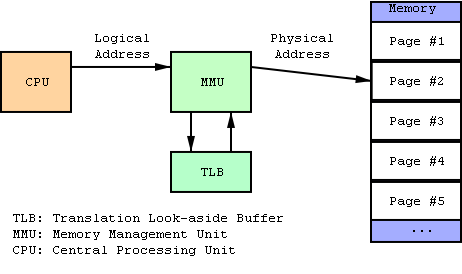
\includegraphics[width=.35\textwidth]{mmu.png}};
    \node at (6,-2) {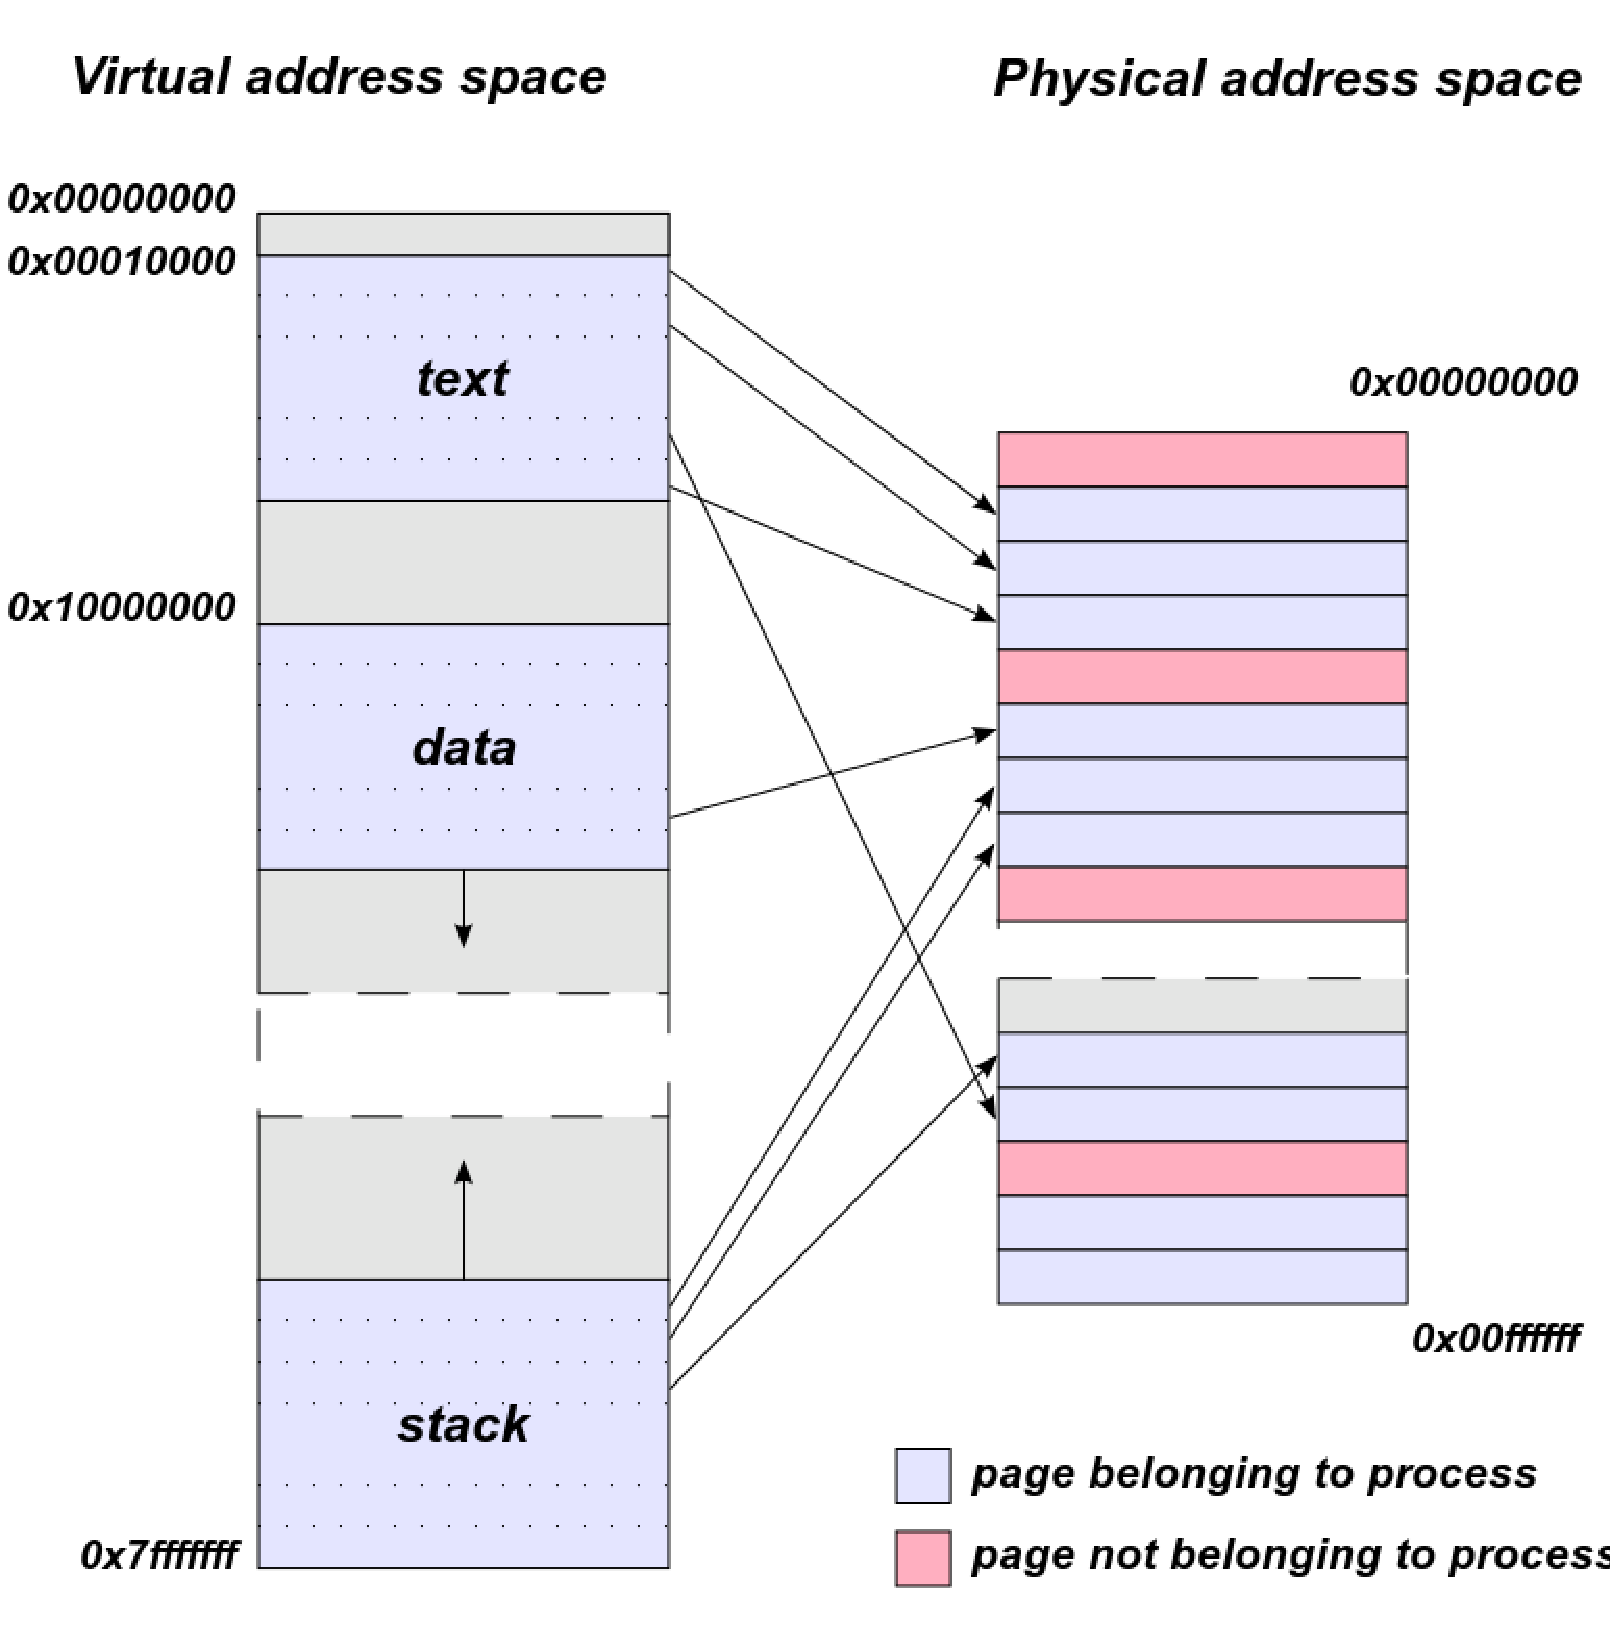
\includegraphics[width=.6\textwidth]{virtualmemory.pdf}};
  \end{tikzpicture}
{\tiny Illustrations from Wikipedia}
\end{frame}


\begin{frame}
  
  \begin{center}
    \Large The memory bandwidth wall
  \end{center}
\end{frame}

\begin{frame}{Benchmarking}

\begin{itemize}
\item<+-> {\bf Problem:} What speed is your CPU {\em really} running at?
  \begin{enumerate}
  \item Power saving
  \item ``Turbo mode''
  \end{enumerate}
\vspace{0.2cm}
\uncover<+->{{\bf Solution:} Disable these features}
\vspace{0.5cm}

\item<+-> {\bf Problem:} Interruptions from the OS\\
\vspace{0.2cm}
\uncover<+->{
  {\bf Solution:} Take many samples of {\em wall time}, then use {\em minimum}. \\
  For each sample, may have to repeat and average.
}
\vspace{0.5cm}

\item<+-> {\bf Problem:} Does benchmark include memory bus etc. or just CPU? \\
\uncover<+->{{\bf Solution:} Benchmark using all CPU cores and with realistically
sized data sets}
\vspace{0.5cm}

\item<+-> {\bf Problem:} The compiler optimizing away the test code

\end{itemize}

\end{frame}

\begin{frame}
Experiments exploring memory bus, cache, cache lines:
\begin{enumerate}
\item<+-> Memory bandwidth
\item<+-> Memory latency
\item<+-> Matrix transpose
\end{enumerate}
\end{frame}

\begin{frame}{Matrix multiplication (Goto \& van de Geijn, 2008)}
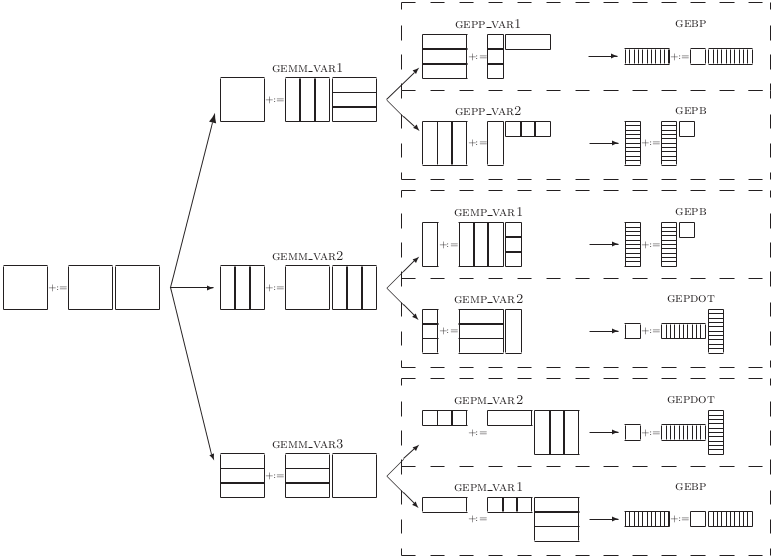
\includegraphics[width=\textwidth]{goto_matmul.png}  
\end{frame}

\begin{frame}
  \begin{center}
    {\Large Parallel computing}
  \end{center}
\end{frame}

\begin{frame}{Multi-core false dependencies (cache line ping pong)}
\uncover<+->{Experiment: {\tt pingpong.c}}
\end{frame}

% \begin{frame}[fragile]{Non-Uniform Memory Architecture}
% \footnotesize
% \only<1>{
% \begin{verbatim}
% Number of nodes: 8
% Memory mask: 0 1 2 3 4 5 6 7 
% Run mask: 0 1 2 3 4 5 6 7 
% #0: Mem: 23.6 GB (22.2 GB free), CPUs: 0 4 8 12 16 20 
% #1: Mem: 23.7 GB (23.5 GB free), CPUs: 24 28 32 36 40 44 
% #2: Mem: 23.7 GB (23.6 GB free), CPUs: 3 7 11 15 19 23 
% #3: Mem: 23.7 GB (20.8 GB free), CPUs: 27 31 35 39 43 47 
% #4: Mem: 23.7 GB (23.2 GB free), CPUs: 2 6 10 14 18 22 
% #5: Mem: 23.7 GB (23.6 GB free), CPUs: 26 30 34 38 42 46 
% #6: Mem: 23.7 GB (22.2 GB free), CPUs: 1 5 9 13 17 21 
% #7: Mem: 23.7 GB (23.3 GB free), CPUs: 25 29 33 37 41 45 
% \end{verbatim}
% }
% \only<2>{fp}
% \end{frame}


\begin{frame}{Competing programming models}
\uncover<+->{
  \begin{itemize}
  \item<+-> MPI: Explicit sharing through message passing (harder, safer)
  \item<+-> OpenMP: Implicit sharing through shared memory (easier, less safe)
  \end{itemize}
}

~

\uncover<+->{
Example: NERSC Hopper cluster
\begin{itemize}
\item 6384 nodes
\item 24 cores per node
\item 32 GB memory per node $\rightarrow$ 1.33 GB per core
\end{itemize}
}

\uncover<+->{
May be better to write 24-threaded program with 32 GB
memory than 1-threaded program with 1.33 GB memory...BUT!
}

~

%\uncover<+->{
%\Large \color{red} If it wasn't for NUMA!!
%}
\end{frame}

\begin{frame}[fragile]{Non-Uniform Memory Architecture}
\footnotesize
\begin{verbatim}
dagss@owl3 $ numactl --hardware
available: 8 nodes (0-7)
node 0 size: 24216 MB
node 0 free: 22685 MB
node 1 size: 24240 MB
node 1 free: 24111 MB
node 2 size: 24240 MB
node 2 free: 24158 MB
<...>
node distances:
node   0   1   2   3   4   5   6   7 
  0:  10  16  16  22  16  22  16  22 
  1:  16  10  16  22  22  16  22  16 
  2:  16  16  10  16  16  16  16  22 
  3:  22  22  16  10  16  16  22  16 
  4:  16  22  16  16  10  16  16  16 
  5:  22  16  16  16  16  10  22  22 
  6:  16  22  16  22  16  22  10  16 
  7:  22  16  22  16  16  22  16  10 
\end{verbatim}
\end{frame}

\begin{frame}[fragile]{Non-Uniform Memory Architecture: AMD}
\footnotesize
\begin{verbatim}
dagss@owl3 $ bin/numabench 6 
== Write (6 threads per node, GiB/s) ==
   5.9     4.9     2.2     1.8     2.1     1.8     4.0     3.6  
   4.9     5.9     2.1     1.8     1.8     2.0     1.9     2.2  
   2.1     2.2     5.9     4.9     2.2     2.2     2.0     1.8  
   2.1     2.1     4.9     5.9     4.0     4.0     1.8     2.1  
   3.7     3.6     2.2     3.9     5.9     4.9     2.2     3.9  
   3.5     3.7     2.2     2.2     4.8     6.0     2.1     3.8  
   2.2     1.9     3.7     3.5     2.2     1.8     5.9     4.9  
   1.8     2.2     1.8     2.1     2.1     1.8     4.9     5.9  
== Read (6 threads per node, GiB/s) ==
  11.1     4.7     2.1     2.0     2.4     2.5     2.1     1.8  
   4.7    11.2     2.1     2.1     2.5     2.4     1.8     2.1  
   2.1     2.1    11.2     4.8     2.1     2.2     2.4     1.7  
   1.8     1.8     4.8    11.1     4.1     2.1     2.5     2.0  
   1.9     1.8     2.1     4.1    11.2     4.4     2.1     2.1  
   1.8     1.9     2.2     2.7     3.2    11.2     1.8     1.8  
   2.6     1.8     1.9     1.7     2.1     2.1    11.1     4.4  
   2.5     2.1     1.7     2.0     2.6     2.3     4.7    11.1  
\end{verbatim}
\end{frame}


\begin{frame}[fragile]{Non-Uniform Memory Architecture: Intel}
\footnotesize
\begin{verbatim}
dagss@mimosa $ bin/numabench 8 
== Write (8 threads per node, GiB/s) ==
  10.1     7.2     5.4     5.1     4.6     5.4     5.3     7.3  
   7.2    10.2     7.7     5.4     5.6     4.6     5.2     5.4  
   5.4     7.6    10.0     7.2     5.4     5.2     4.5     5.5  
   5.1     5.4     7.2    10.0     7.3     5.4     5.4     4.5  
   4.5     5.4     5.3     7.2    10.0     7.2     5.4     5.1  
   5.5     4.5     5.2     5.4     7.2    10.0     7.6     5.4  
   5.3     5.2     4.5     5.5     5.4     7.6    10.0     7.2  
   7.3     5.3     5.4     4.5     5.1     5.4     7.2    10.0  
== Read (8 threads per node, GiB/s) ==
  22.0     7.6     8.2     7.4     7.1     7.8     8.0     8.5  
   7.7    21.9     8.6     8.2     7.3     7.0     7.5     8.0  
   8.1     9.0    21.8     7.6     8.0     7.4     7.0     7.4  
   7.3     8.1     7.6    22.0     9.4     8.0     7.7     6.9  
   7.0     7.7     7.9     9.2    21.9     7.6     8.2     7.3  
   7.4     6.9     7.4     7.9     7.6    21.8     8.9     8.2  
   8.0     7.5     7.0     7.3     8.1     8.6    21.8     7.6  
   9.0     8.0     7.7     6.9     7.3     8.1     7.6    22.0  
\end{verbatim}
\end{frame}

\begin{frame}{Hybrid approach!}

NERSC:
\begin{quote}
  When using hybrid OpenMP-MPI in applications NERSC strongly suggests
  running with 4 MPI tasks and 6 OpenMP threads each per node.  Using
  1 MPI task and 24 OpenMP threads per node is NOT an optimal way to
  use the Hopper nodes, as it is very hard to address the performance
  implications of the Non-Uniform Memory Architecture (NUMA) of the
  Hopper nodes using more than 6 OpenMP threads.
\end{quote}
{\small \tt http://1.usa.gov/UuFzYe}

~

{\tt numactl} is your friend!
\end{frame}

\begin{frame}{Summary and opinions on parallelism}
\begin{itemize}
  \item<+-> Sharing memory is convenient but dangerous for performance
  \item<+-> Does OpenMP make it too easy to share memory?
  \item<+-> Non-trivial code: Dead-locks, races, ...
  \item<+-> Alternative 1: Asynchronous message passing with ZeroMQ!
    \begin{itemize}
    \item Beautiful programming interface!
    \item Extremely fast
    \item In-process, cross-process, cluster, or internet
    \end{itemize}
    
\includegraphics[width=0.3\textwidth]{zeromq.png}
  \item<+-> Alternative 2 (experts): Use MPI and explicitly share memory on same
     node
     \begin{itemize}
     \item {\tt man shmem}
     \item {\tt man mmap}
     \end{itemize}
   \item<+-> Alternative $n$: Too many frameworks to even begin...
\end{itemize}

\end{frame}

\begin{frame}
  \begin{center}
    \LARGE A more complicated picture of CPUs

~

(+ some GPU)
  \end{center}
\end{frame}

\begin{frame}{CPUs getting more complicated}
  \begin{center}
    \only<1>{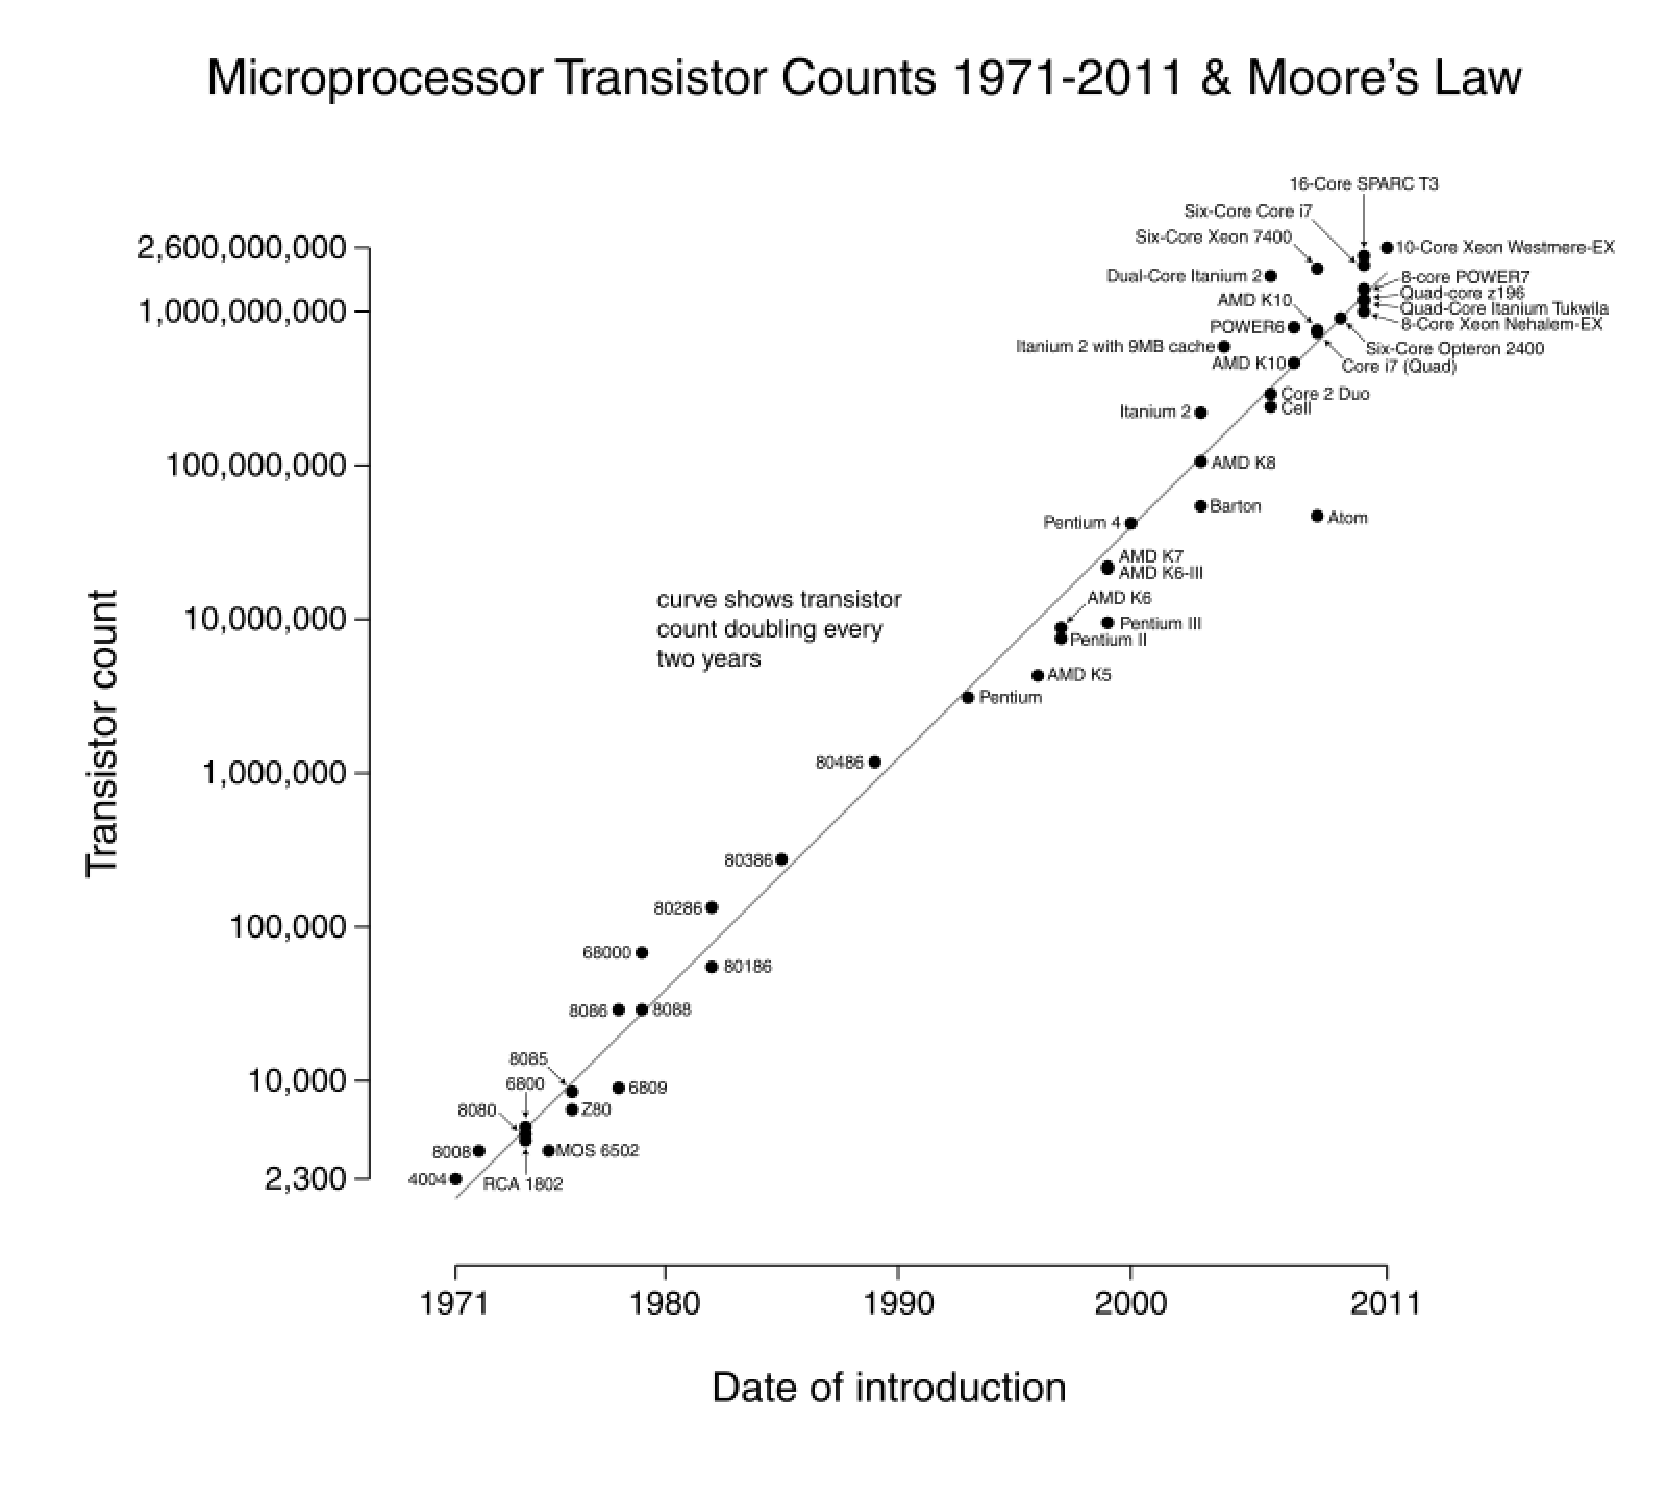
\includegraphics[width=0.8\textwidth]{transistors.pdf}}
    \only<2>{But:\\[5mm]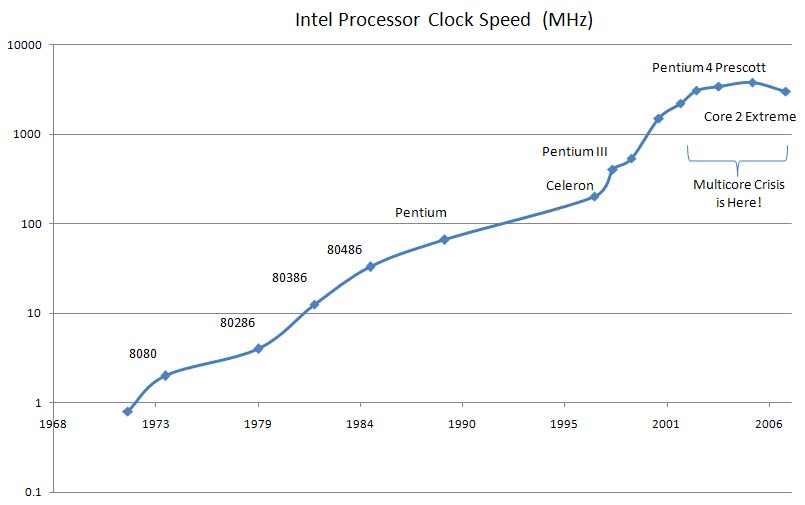
\includegraphics[width=0.8\textwidth]{clockspeeds.jpg}}
  \end{center}
  
\end{frame}

\begin{frame}{CPUs today}
  \begin{center}
    \only<1>{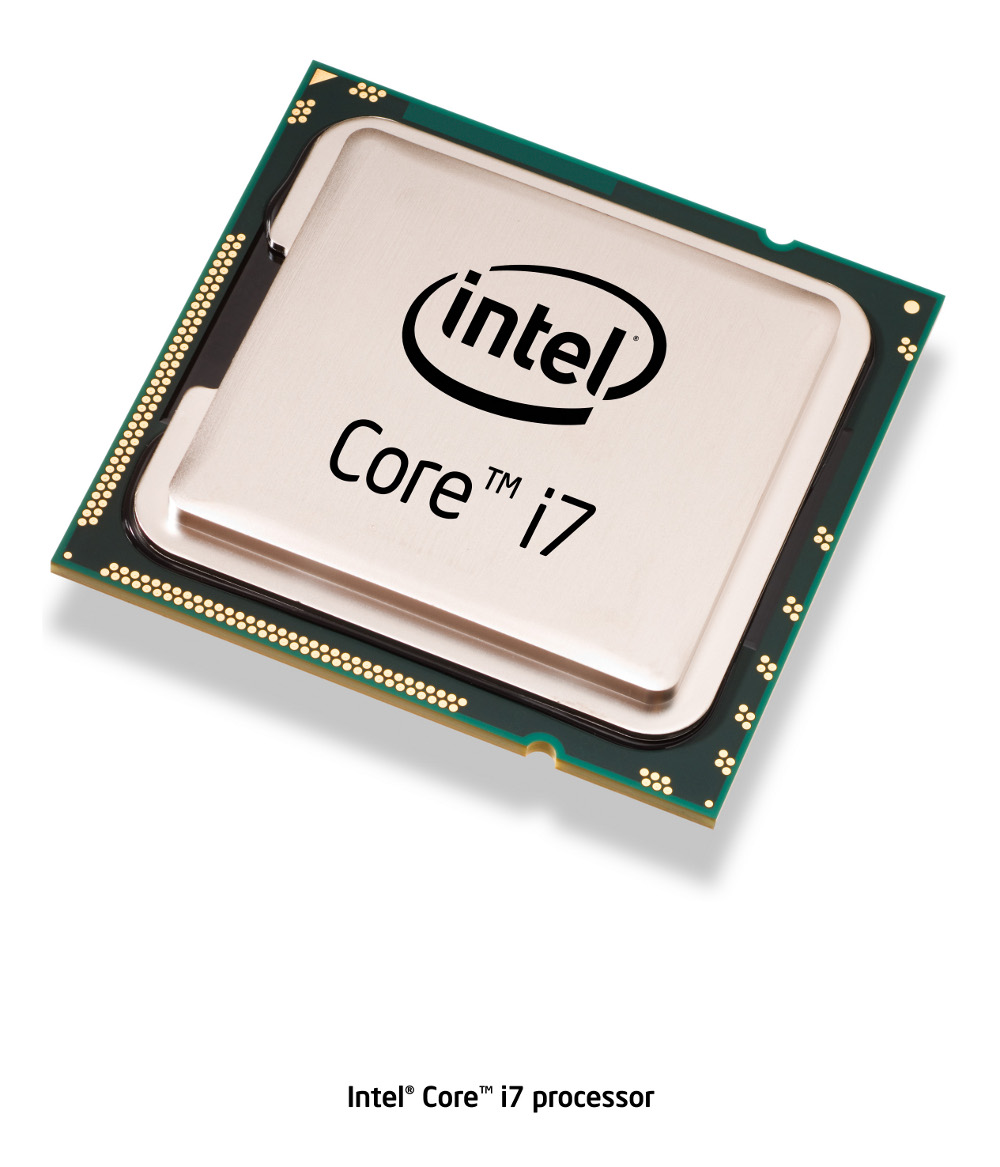
\includegraphics[width=0.8\textwidth]{nehalem_front.jpg}}
    \only<2>{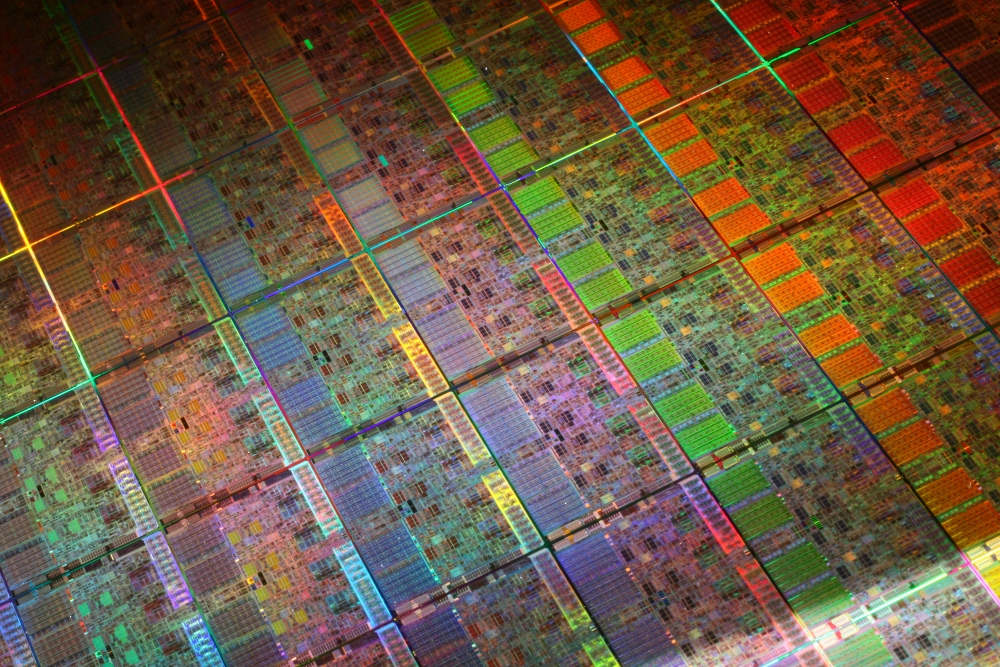
\includegraphics[width=0.8\textwidth]{nehalem_wafer.jpg}}
    \only<3>{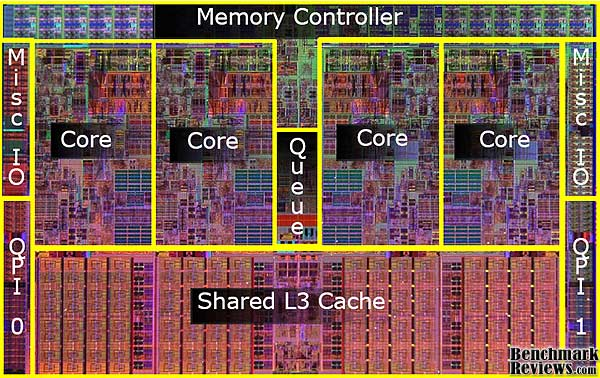
\includegraphics[width=0.8\textwidth]{nehalem_callout.jpg}}
  \end{center}
\end{frame}
\begin{frame}
  \begin{center}
    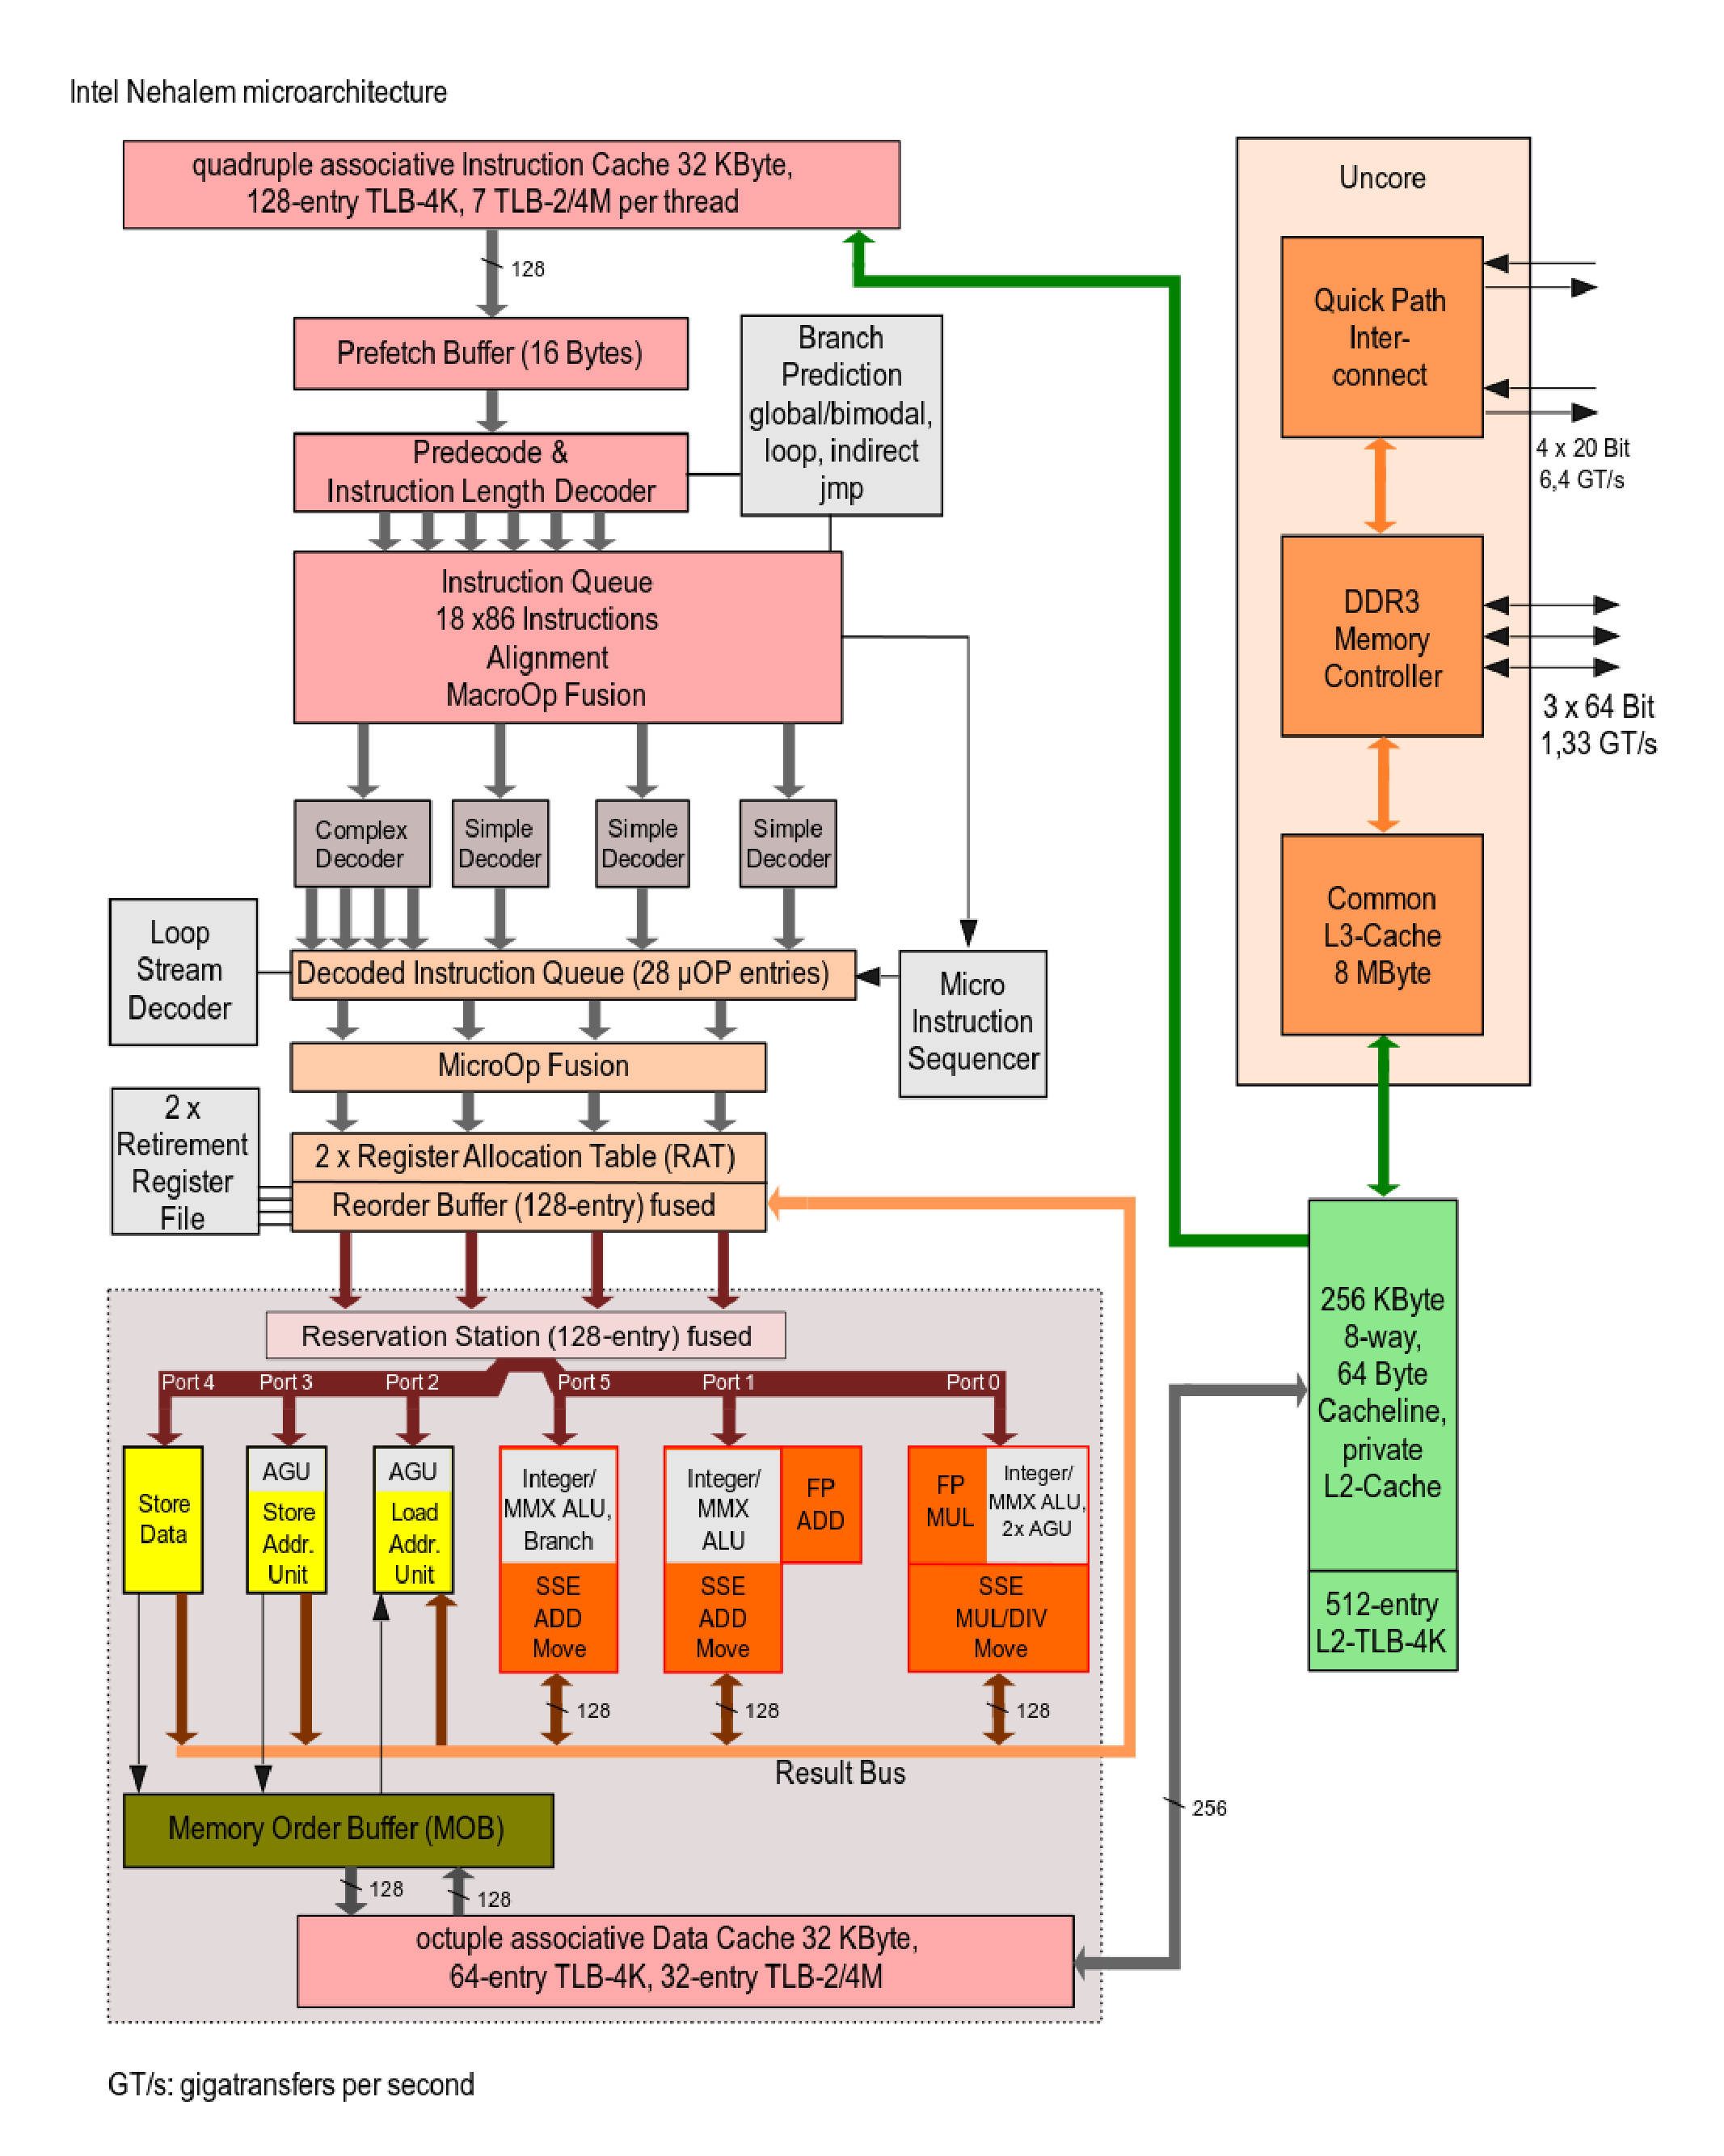
\includegraphics[height=\textheight]{nehalem_arch.pdf}
  \end{center}
\end{frame}
\begin{frame}
  \begin{center}
    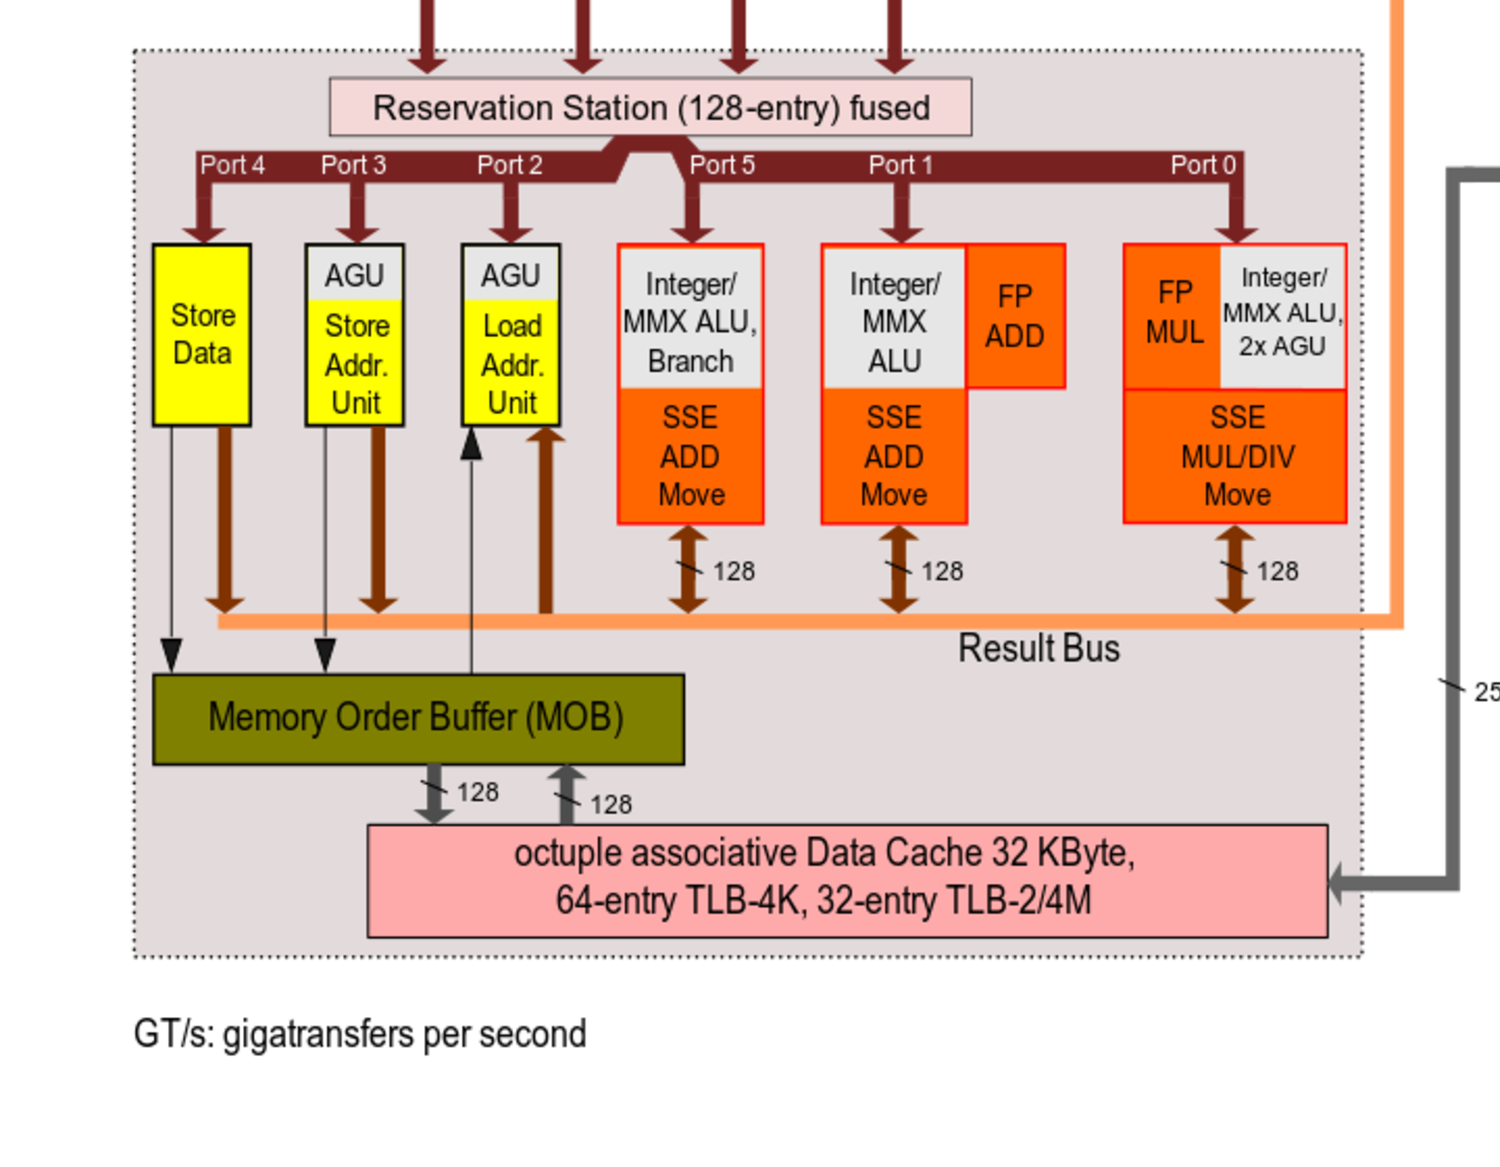
\includegraphics[height=\textheight]{nehalem_arch_crop.pdf}
  \end{center}
\end{frame}

\begin{frame}[fragile]{Out-of-order execution \& register renaming}
  \begin{tikzpicture}
    \node[text width=8cm]{
\begin{verbatim}
mov    eax, [rsp]
imul   eax, eax
mov    [rsp], eax
mov    eax, [rsp+0x4]
imul   eax, eax
mov    [rsp+0x4], eax
\end{verbatim}

% will execute more similar to:

% \begin{verbatim}
% mov    eax0, [rsp]
% mov    eax1, [rsp+0x4]
% imul   eax0, eax0
% imul   eax1, eax1
% mov    [rsp], eax0
% mov    [rsp+0x4], eax1
% \end{verbatim}

    };
    \node at (4, -2) {
      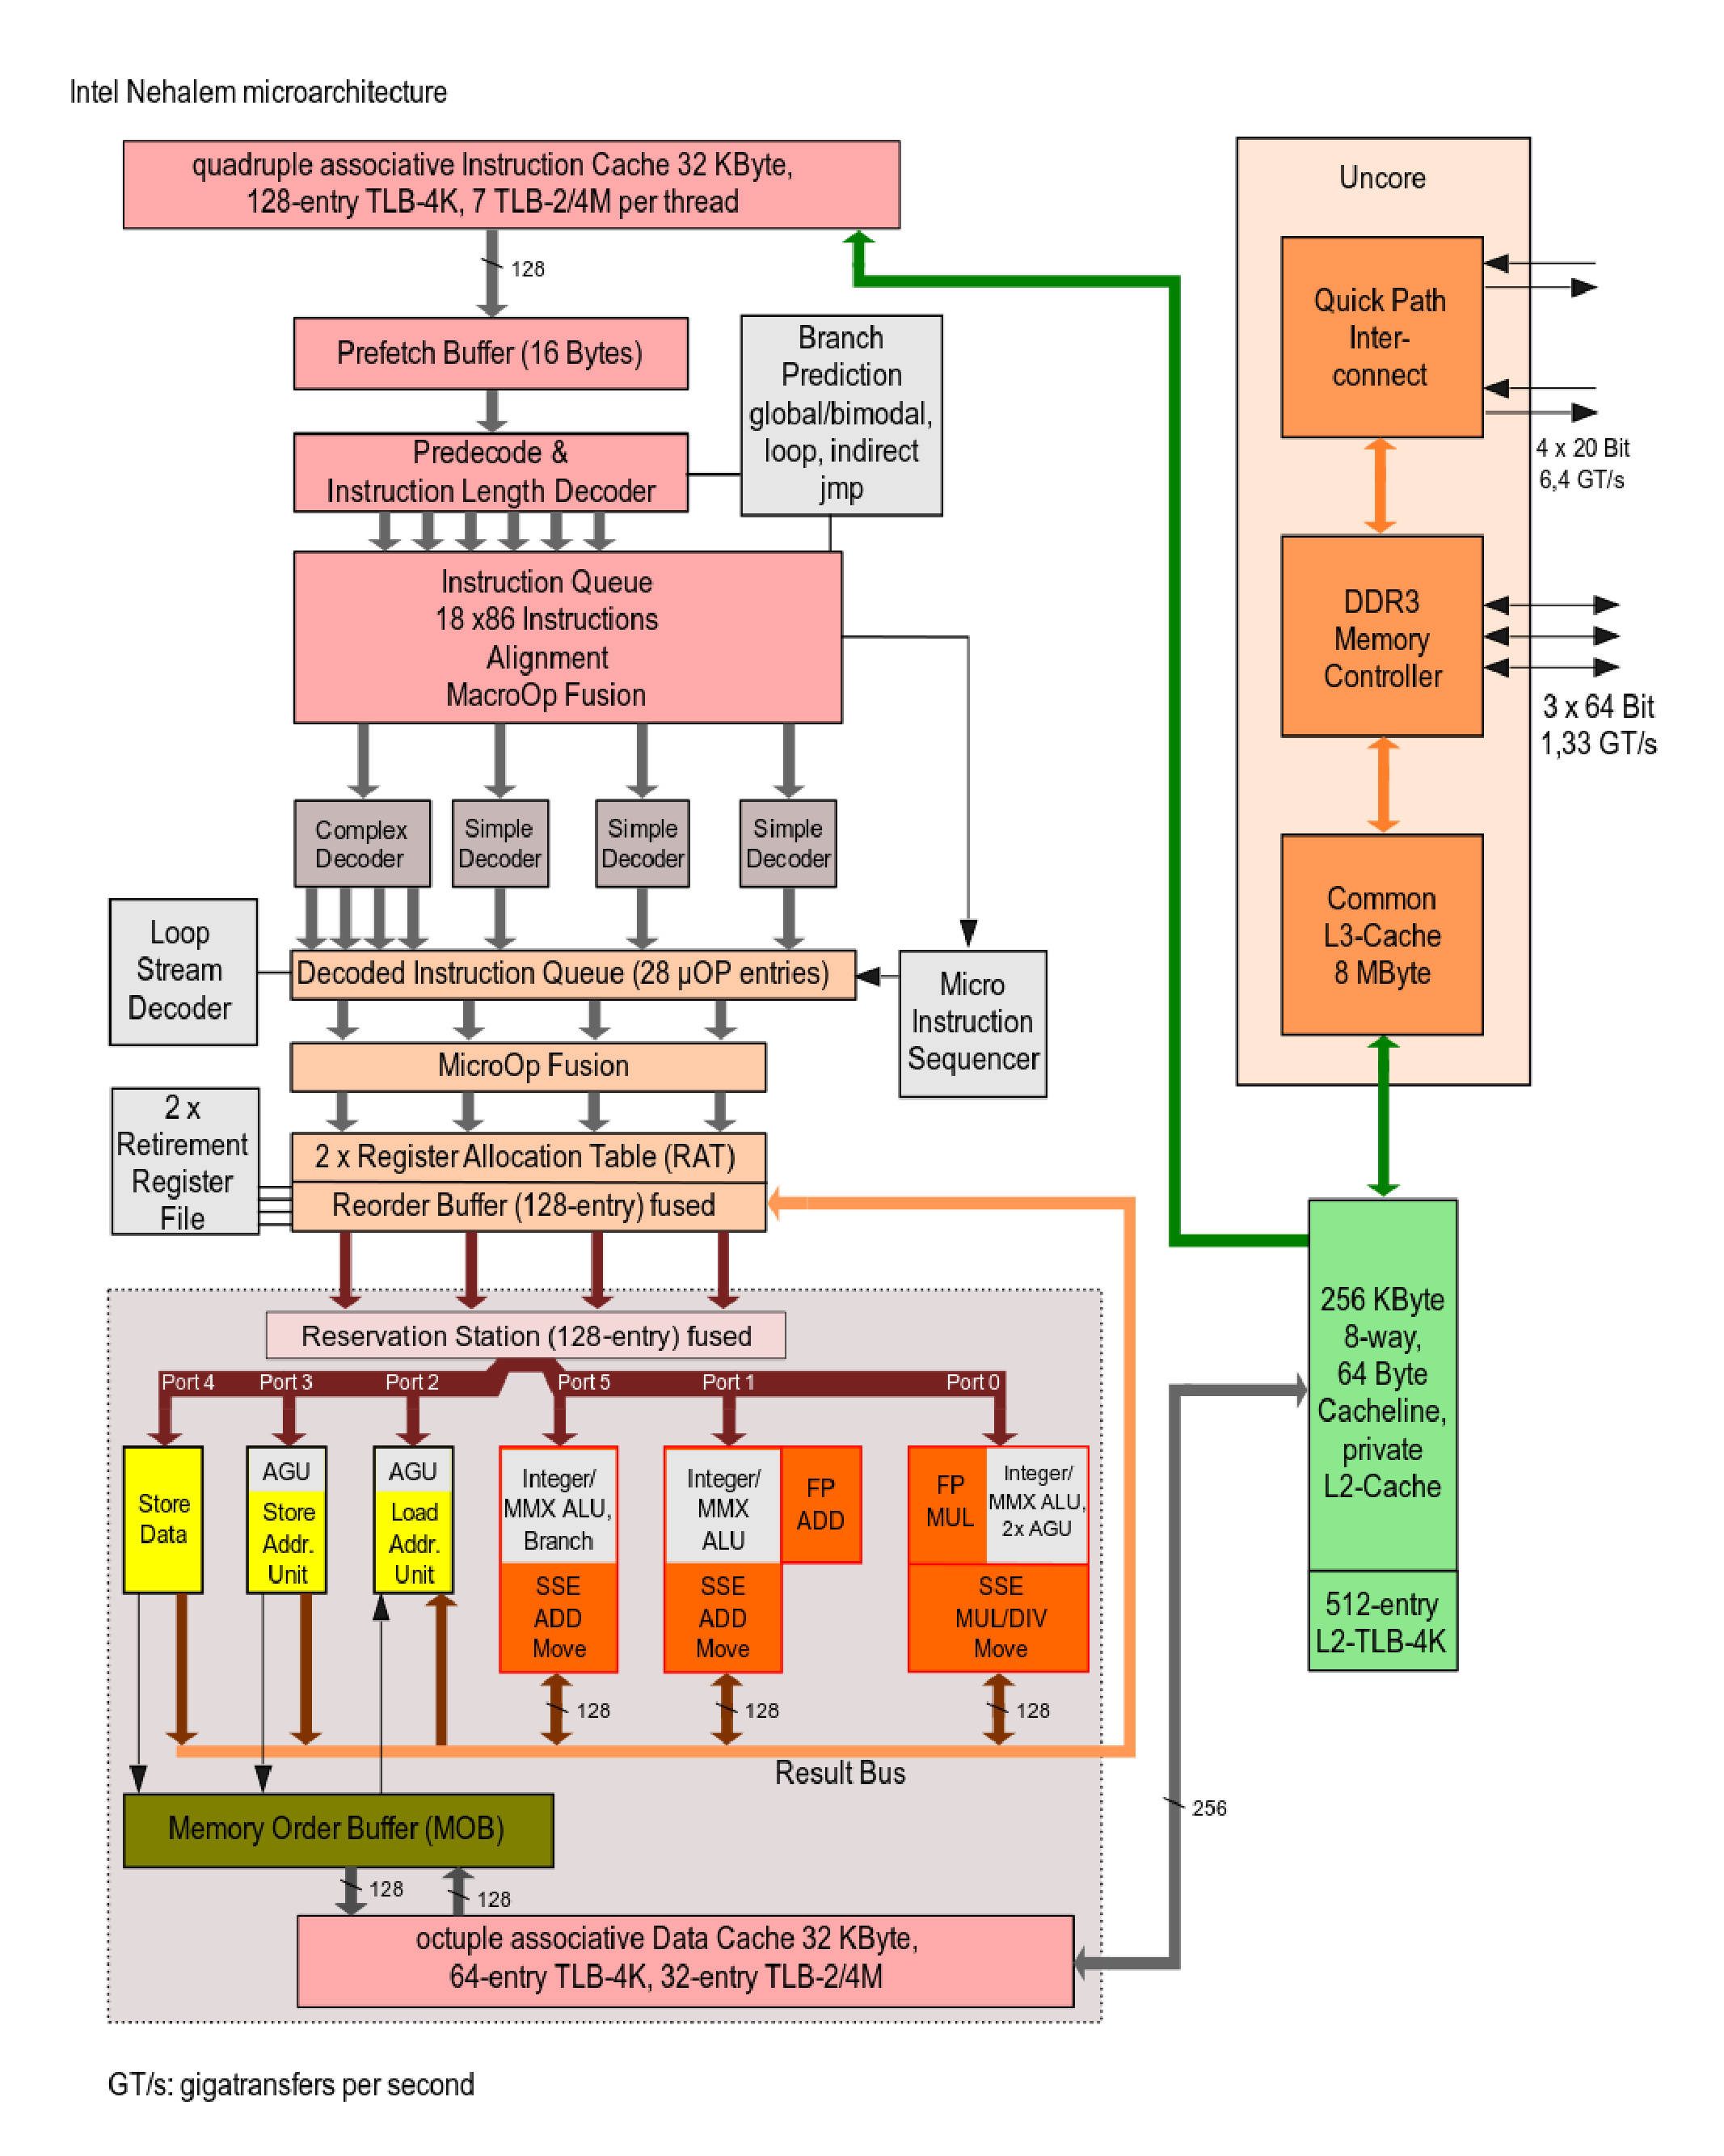
\includegraphics[width=0.6\textwidth]{nehalem_arch.pdf}
    };
  \end{tikzpicture}
\end{frame}

\begin{frame}[fragile]{Pipelining}
  \begin{tikzpicture}
    \node[text width=8cm]{
Not so good:
{\small
\begin{verbatim}
for (i = 2; i < n; ++i) {
    out[i] = a[i] * out[i - 2] + b[i] * out[i - 1];
}
\end{verbatim}
}

~

Good:
{\small
\begin{verbatim}
for (i = 0; i < n; ++i) {
    out[i] = a[i] + b[i];
}
\end{verbatim}
}
    };
    \node at (4.5, -3) {
      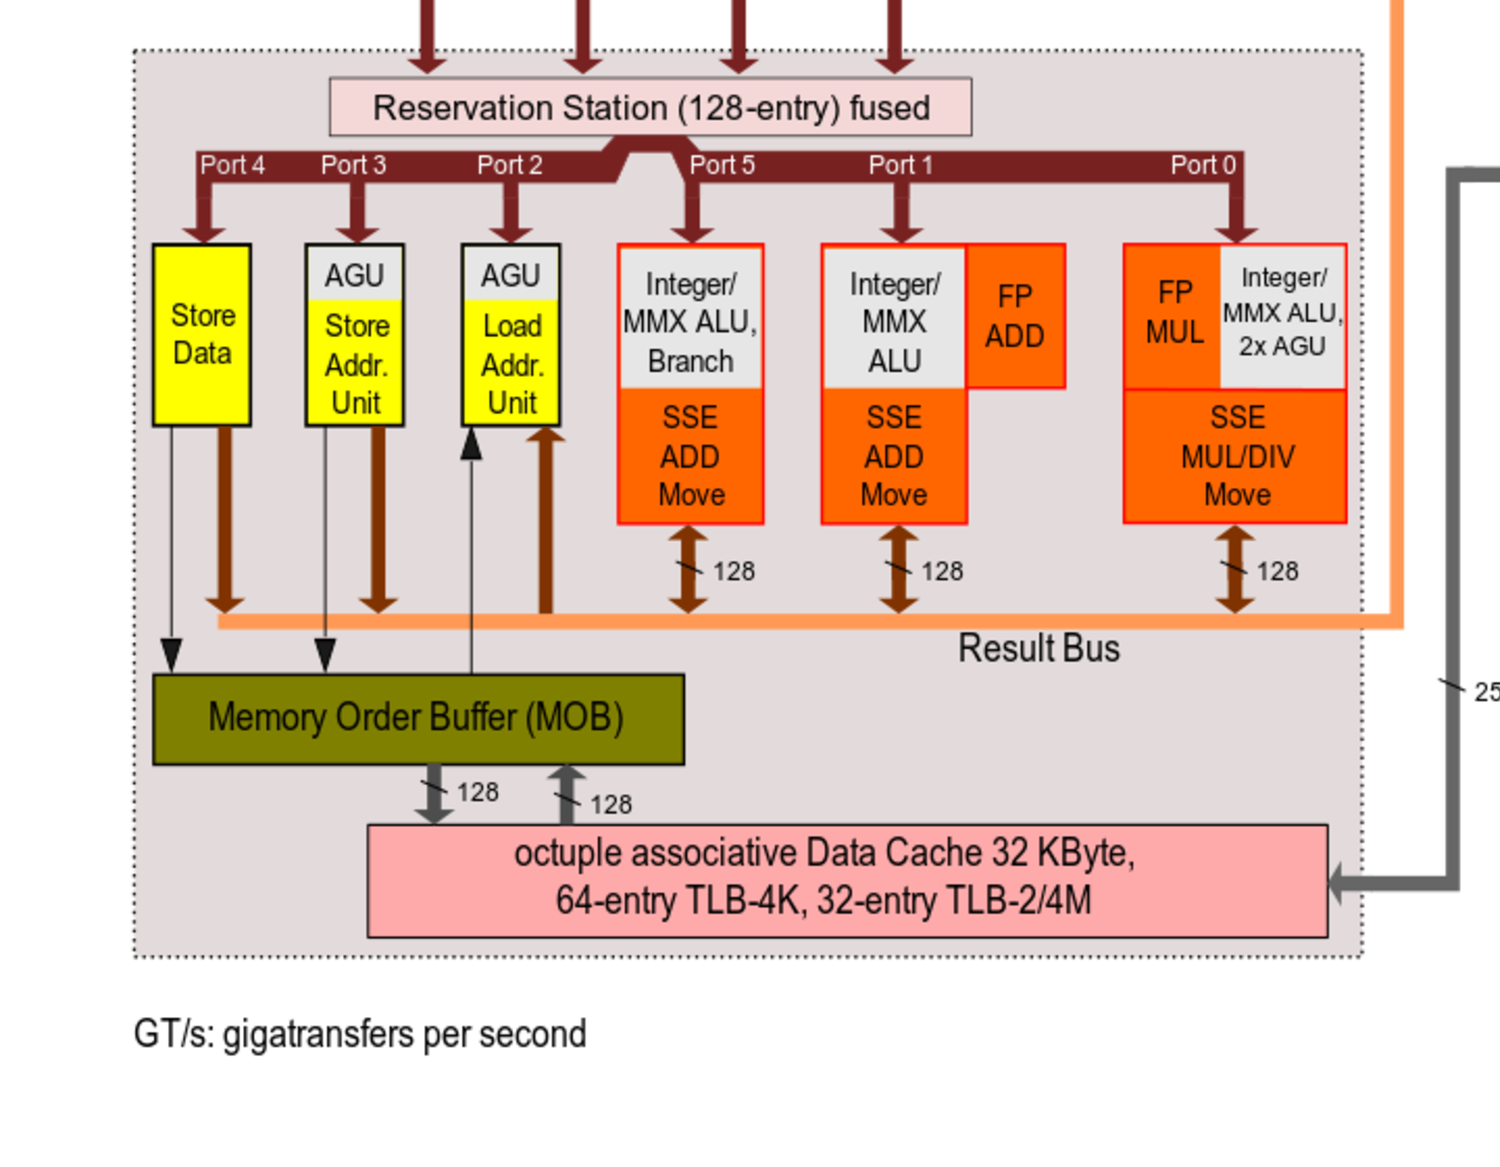
\includegraphics[width=0.7\textwidth]{nehalem_arch_crop.pdf}
    };
  \end{tikzpicture}
\end{frame}


\begin{frame}[fragile]{Branch prediction \& speculative execution}
  \begin{tikzpicture}
    \node[text width=8cm]{
\begin{verbatim}
x = f(y);
if (x < 100) {
    x *= 2;
} else {
   x -= 100;
}
\end{verbatim}

    };
    \node at (4.5, -3) {
      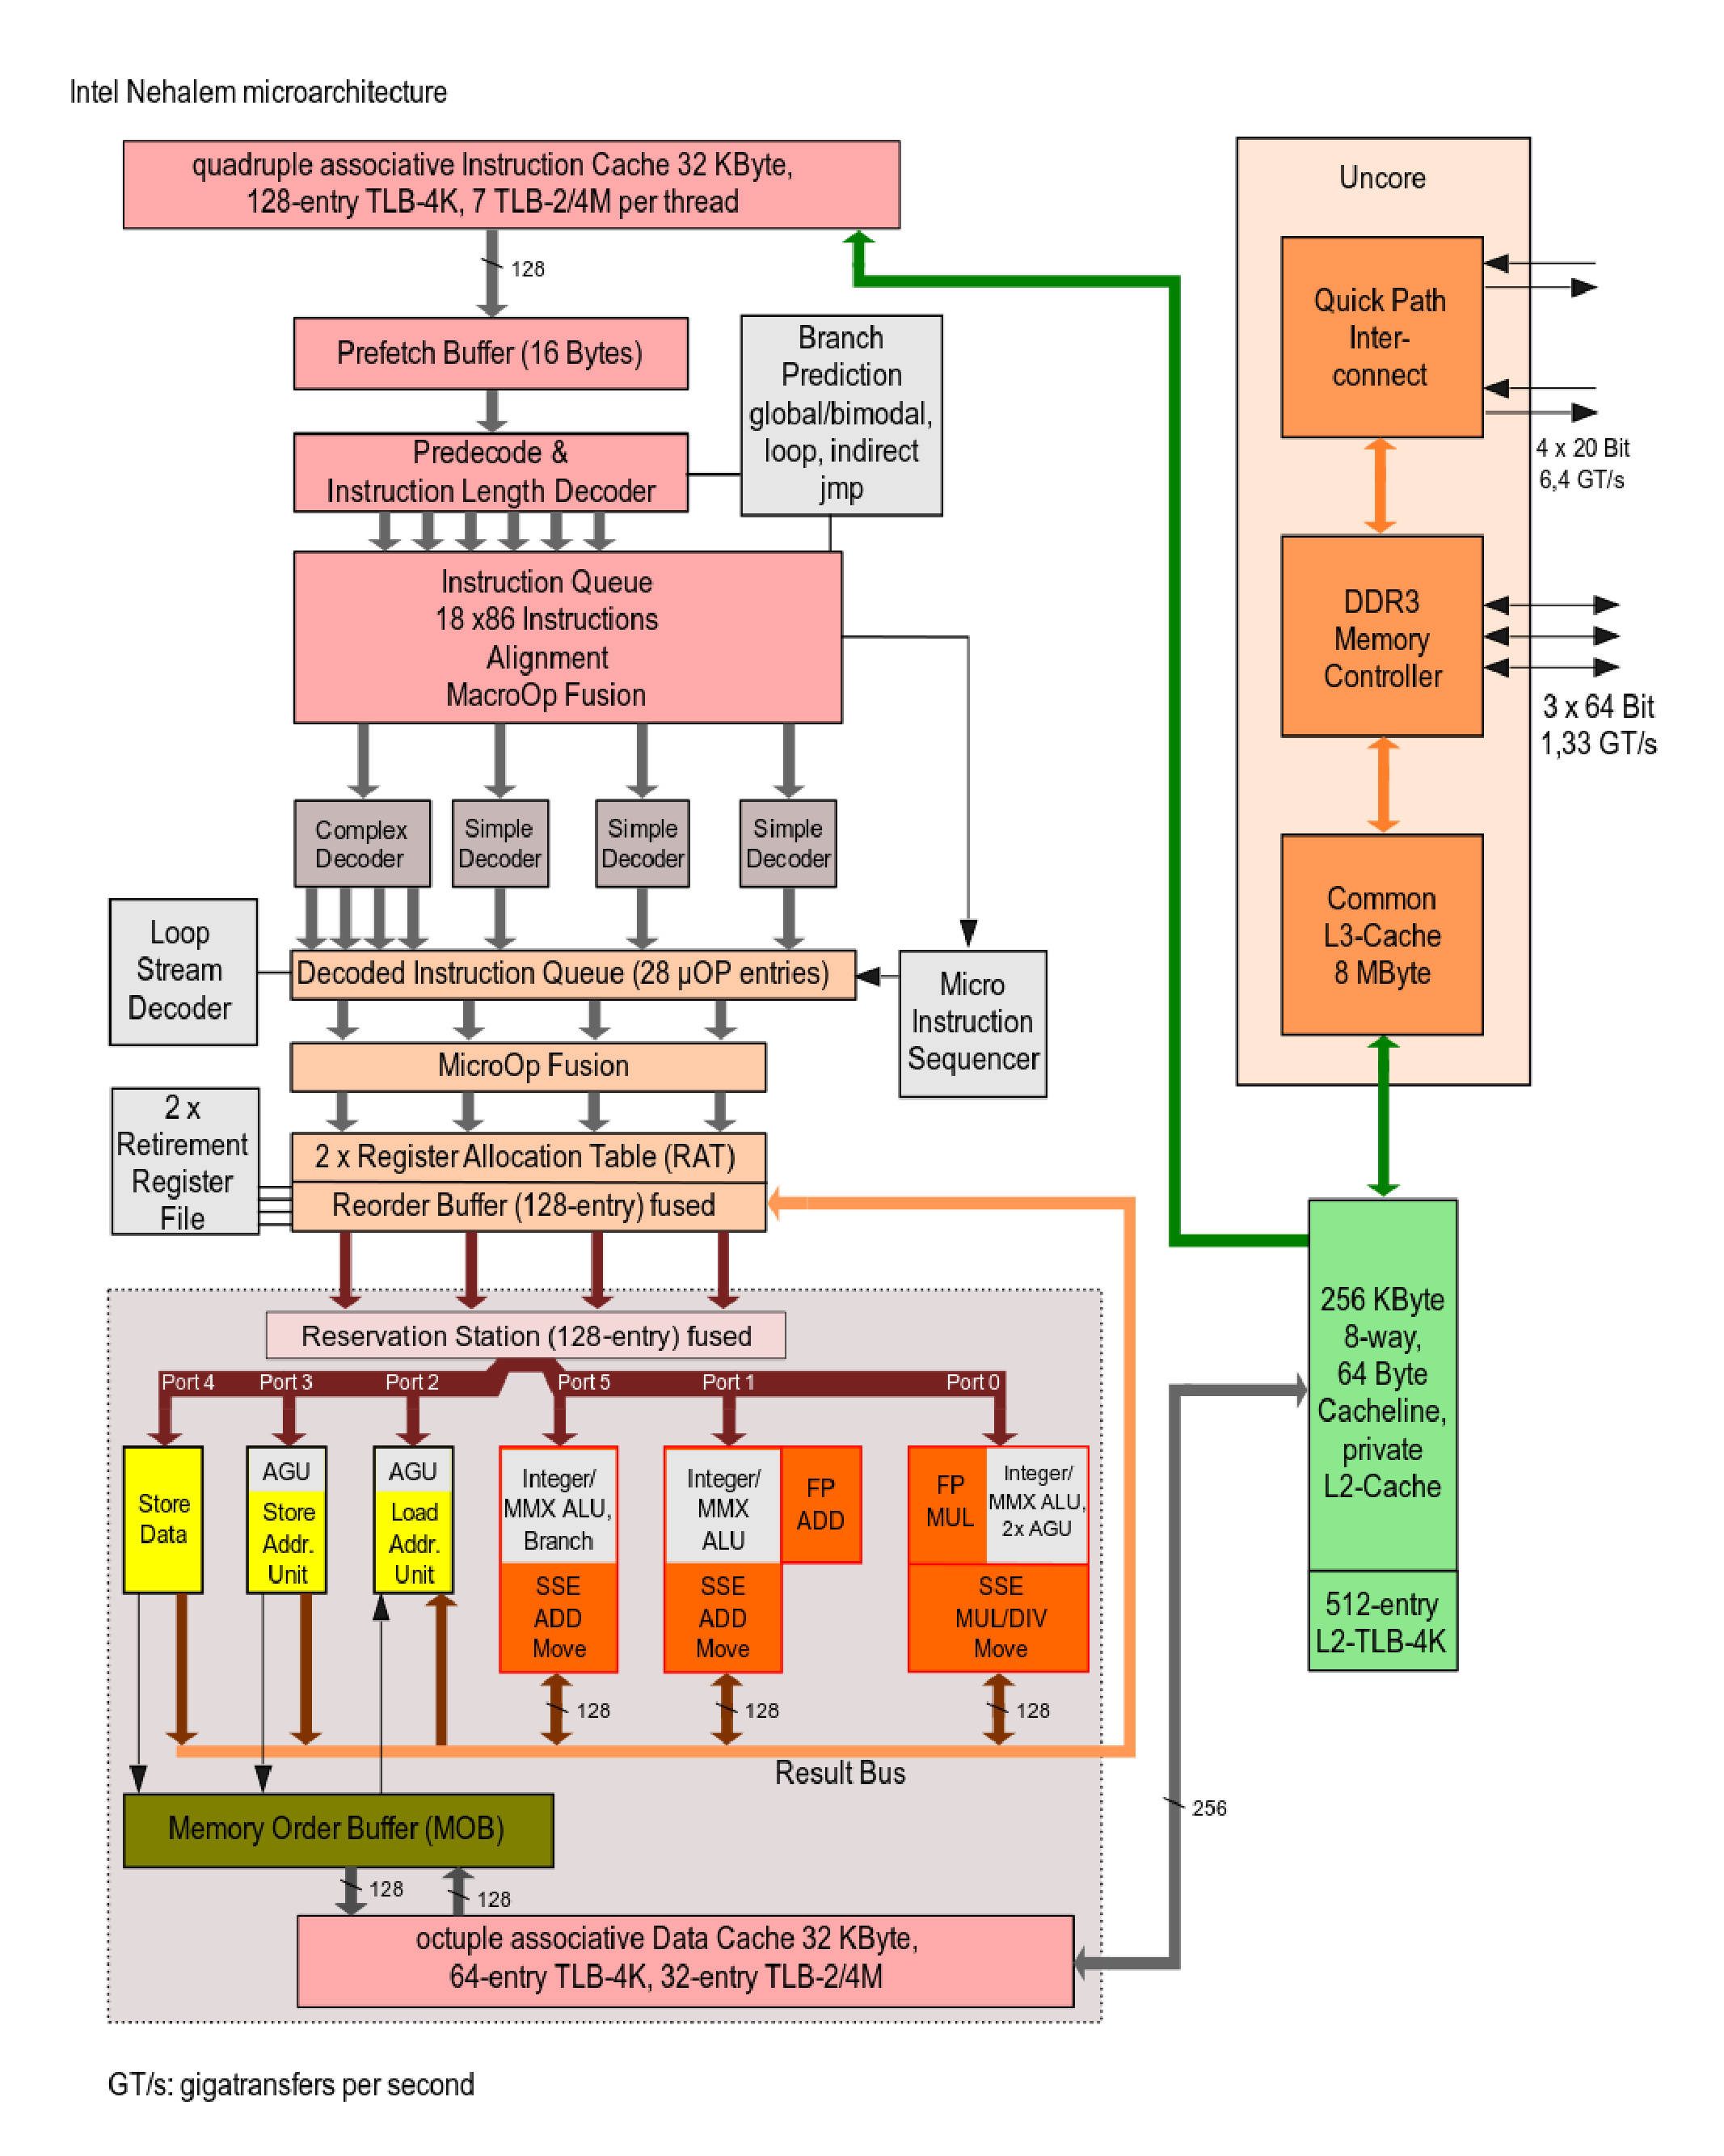
\includegraphics[width=0.6\textwidth]{nehalem_arch.pdf}
    };
  \end{tikzpicture}
\end{frame}

\begin{frame}{Vector instructions}
  \begin{itemize}
  \item SSE: 128-bit registers (4 $\times$ SP or 2 $\times$ DP)
  \item AVX: 256-bit registers (8 $\times$ SP or 4 $\times$ DP)
  \end{itemize}

~

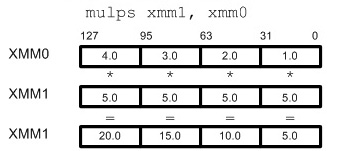
\includegraphics[width=.6\textwidth]{sse.jpg} 

~

Experiment: {\tt sse\_transpose.c}
\end{frame}

\begin{frame}{Example}

Legendre transform:
\[
q_{i} = \sum_{k = k_\mathrm{start}}^{k_\mathrm{stop}} \Lambda_{i,k} a_{k}
\]


\end{frame}

\renewcommand{\P}{\widetilde{P}}
\begin{frame}
  \frametitle{The Legendre functions by recurrence relation}

 \begin{equation*}
    \begin{split}
        \Lambda_{i,k+1} =& (x_i^2 + \alpha_{k}) \beta_{k} \Lambda_{i,k}
        + \gamma_{k} \Lambda_{i,k-1}
      \end{split}
    \end{equation*}

  \begin{center}
    \begin{tikzpicture}
      \node{
      \only<1>{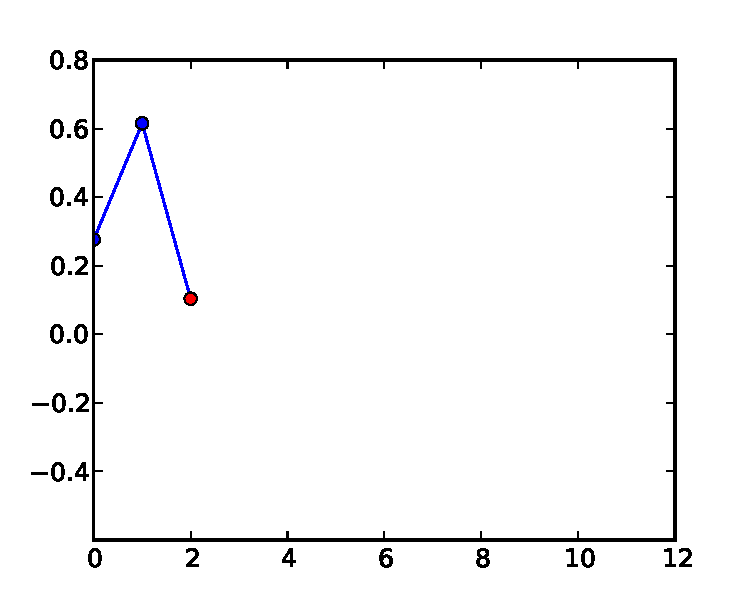
\includegraphics[width=.5\textwidth]{P3.pdf}}%
      \only<2>{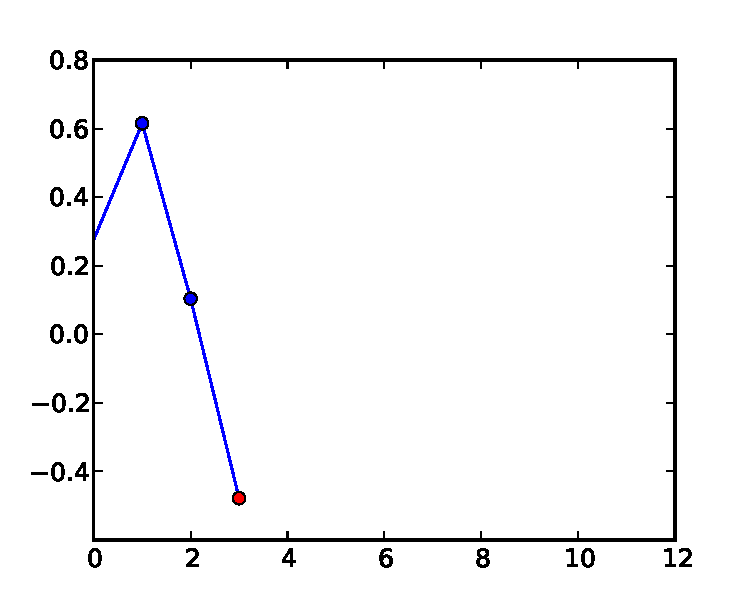
\includegraphics[width=.5\textwidth]{P4.pdf}}%
      \only<3>{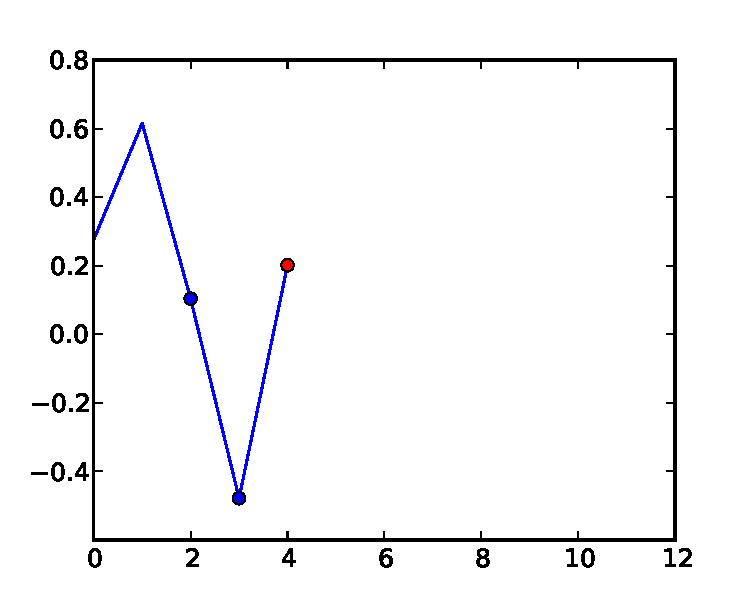
\includegraphics[width=.5\textwidth]{P5.pdf}}%
      \only<4>{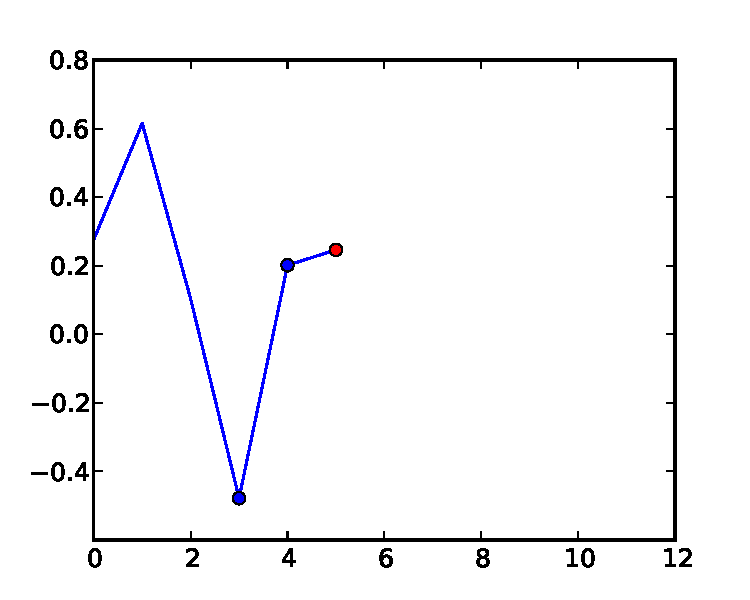
\includegraphics[width=.5\textwidth]{P6.pdf}}%
      \only<5>{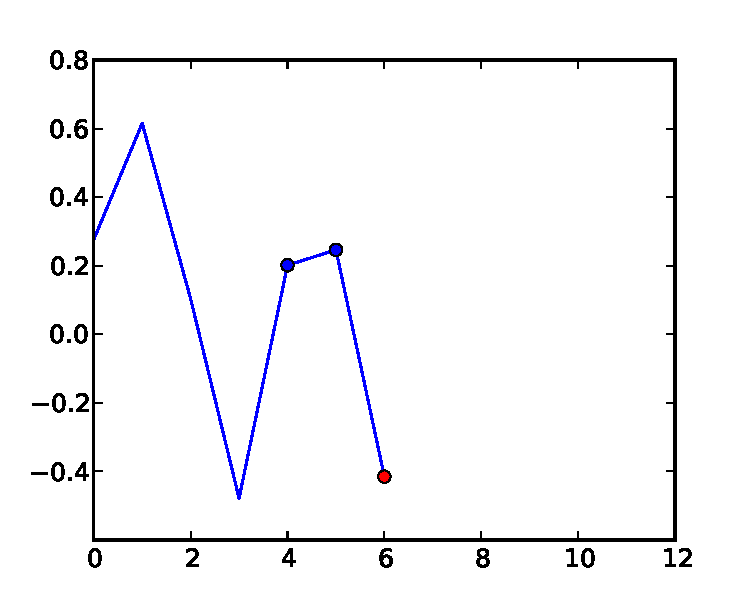
\includegraphics[width=.5\textwidth]{P7.pdf}}%
      \only<6>{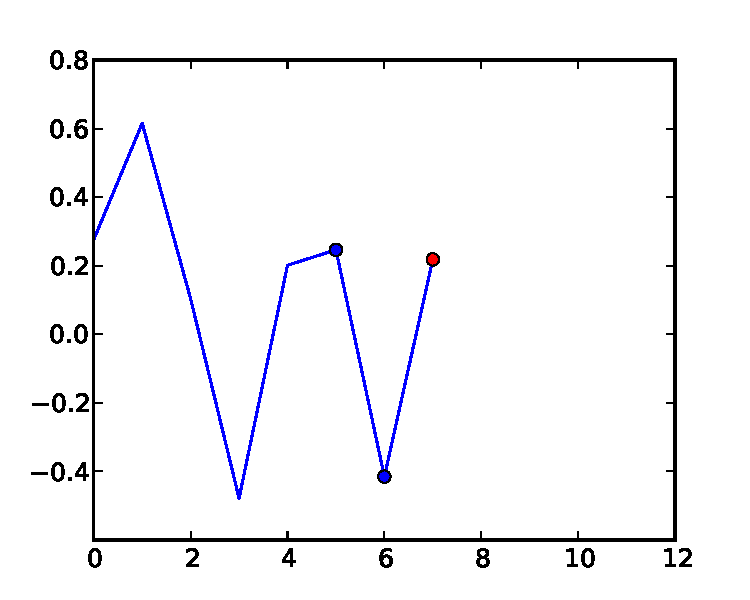
\includegraphics[width=.5\textwidth]{P8.pdf}}%
      \only<7>{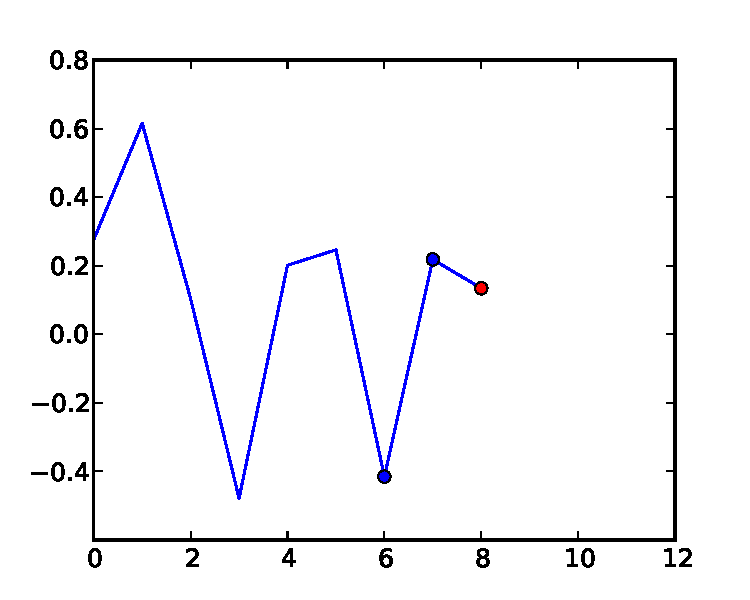
\includegraphics[width=.5\textwidth]{P9.pdf}}%
      \only<8>{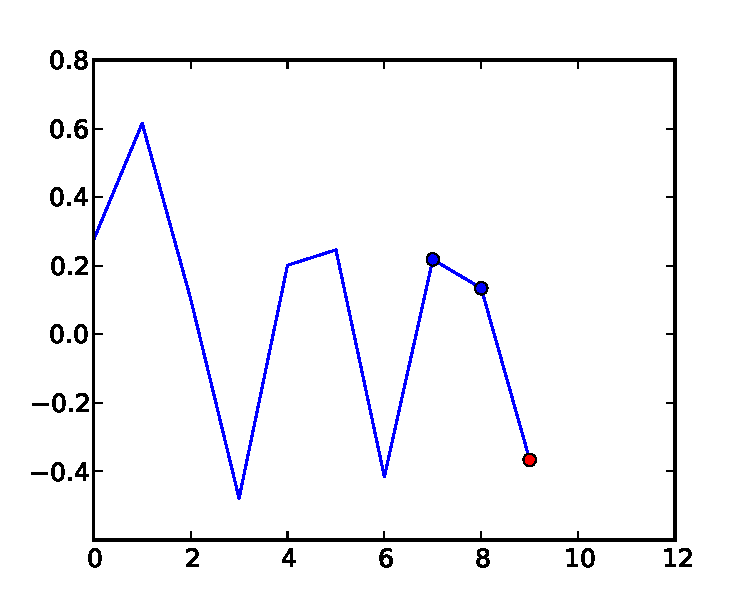
\includegraphics[width=.5\textwidth]{P10.pdf}}%
      \only<9>{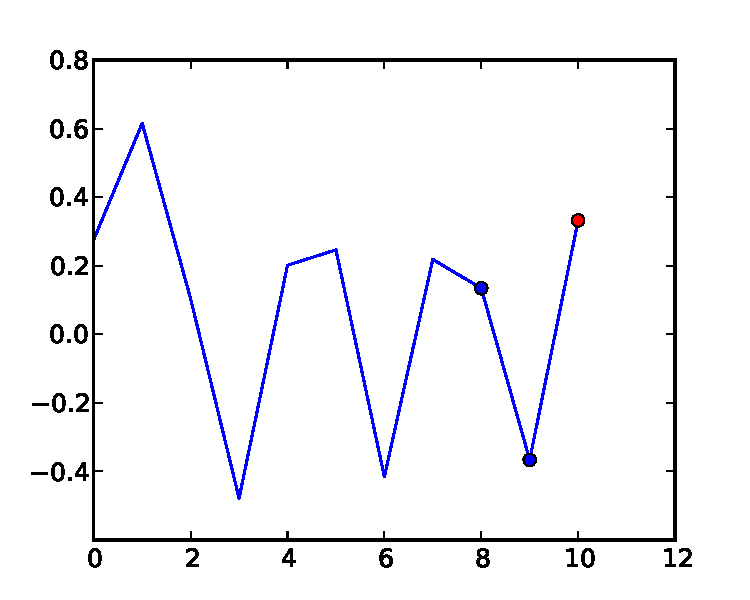
\includegraphics[width=.5\textwidth]{P11.pdf}}};

%      \node[text width=5cm,anchor=west] at (3cm, 0) {
%        \small
%        We want to compute
%        \[
%        q_{i} = \sum_{k = k_\mathrm{start}}^{k_\mathrm{stop}} \Lambda_{i,k} a_{k}
%        \]
%      };
    \end{tikzpicture}
  \end{center}

 
%E.g.,
%{\footnotesize
%\[\beta_{k} =
%      \sqrt{\frac{(4k + 1)(4k +3)^2(4k + 5)} {(2k - m + 1)(2k - m +
%          2)(2k + m + 1)(2k + m + 2)}}
%\]
%}
\end{frame}

\newcommand{\gridsize}{3mm}

\begin{frame}
  \frametitle{Legendre transform}
  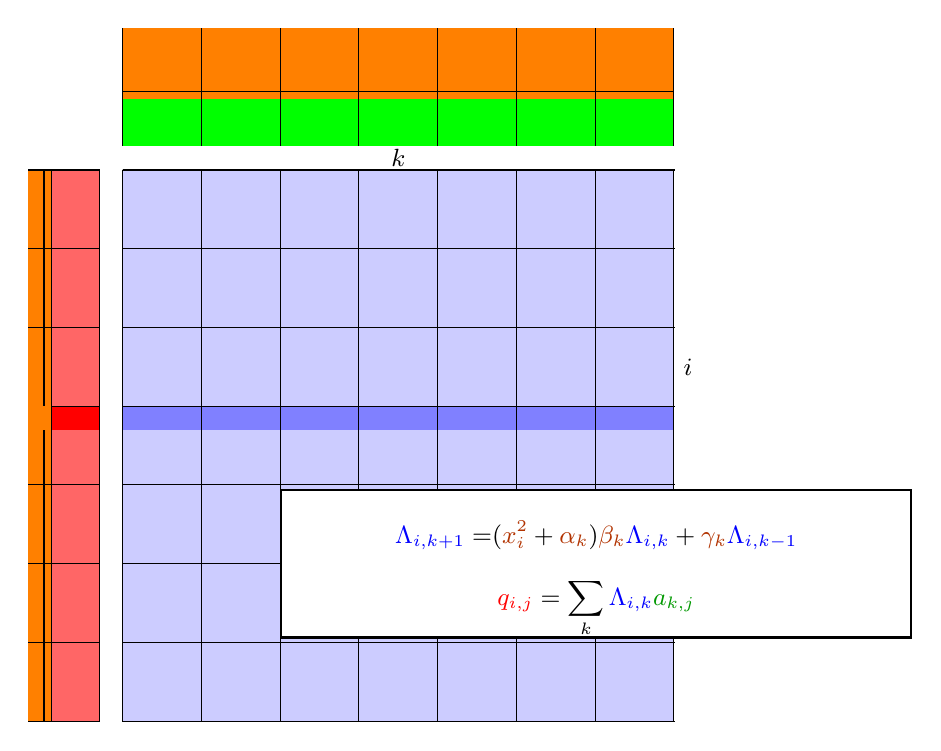
\begin{tikzpicture}[yscale=-1]

    %
    % Lambda
    %
    \node[fill=blue!20,minimum width=7cm,minimum height=7cm,anchor=north west] (Lambda) {
    };

    \draw (0,0) -- (7cm, 0cm) node[midway,anchor=south,outer sep=0,inner sep=.5mm] {\small $k$};
    \draw (7cm,0cm) -- (7cm, 5cm) node[midway,anchor=west] {\small $i$};

    \fill[blue!50] (0,30mm) rectangle (7cm,33mm);

    \draw (Lambda.north west) grid[step=\gridsize] (Lambda.south east);
    \coordinate (a) at (0,0);
    \coordinate (ap) at (0,7);
    \coordinate (b) at (3.9,0);
    \coordinate (bp) at (3.9,7);
    \coordinate (c) at (0,1.95);
    \coordinate (cp) at (7,1.95);
    \coordinate (d) at (0,4.05);
    \coordinate (dp) at (7,4.05);

    % \draw[fill=blue!40] ($(c)!(a)!(cp)$) rectangle ($(d)!(b)!(dp)$);
    % \fill[fill=red!60!blue] ($(a)!(c)!(ap)$) rectangle ($(b)!(c)!(bp) - (0,3mm)$);
    % \draw ($(c)!(a)!(cp) - (0,3mm)$) grid[step=\gridsize] ($(d)!(b)!(dp)$);

    % \draw[thick,decorate,decoration={brace,amplitude=2mm}]
    %    ($(b)!(c)!(bp)$) -- ($(b)!(d)!(bp)$)
    %    node[fill=white,midway,anchor=west,inner sep=2pt, outer sep=6pt]{\footnotesize $B_k$};

    % \draw[thick,decorate,decoration={brace,amplitude=2mm}]
    %    ($(b)!(d)!(bp)$) -- ($(a)!(d)!(ap)$)
    %    node[fill=white,midway,anchor=north,inner sep=2pt, outer sep=6pt]{
    %      \footnotesize $B_i \times n_\mathrm{threads}$};

    %\node[yscale=3,anchor=north]  {$\Big\}$};


    %
    % i-wise
    %
    
    \node[fill=orange,minimum width=3mm,minimum height=7cm,anchor=north east,outer sep=0,%
    inner sep=0,shift={(-9mm,0)}] (aux) at
      ($(Lambda.north west)$) {};
    \draw (aux.north west) grid[step=\gridsize] (aux.south east);

    \fill[orange] (-12mm,30mm) rectangle (-9mm, 33mm);
    
    \node[draw,fill=red!60,minimum width=6mm,minimum height=7cm,anchor=north east,outer sep=0,%
    inner sep=0,shift={(-3mm,0)}] (A) at
      (Lambda.north west) {};

    \fill[red] (-9mm,30mm) rectangle (-3mm, 33mm);
    \draw[black] (A.north west) grid[step=\gridsize] (A.south east);

    % k-wise
    \node[fill=green,minimum width=7cm,minimum height=6mm,anchor=south west] (Q) at
      ($(Lambda.north west) - (0,3mm)$) {};
    \draw (Q.north west) grid[step=\gridsize] (Q.south east);

    \coordinate (xsq-a) at ($(Lambda.north west) - (0,9mm) - (0, 6mm) - (0, 3mm)$);
    \coordinate (xsq-b) at ($(xsq-a) + (7cm,0)$);
    \coordinate (xsq-c) at ($(xsq-a) + (7cm,9mm)$);
    \coordinate (xsq-d) at ($(xsq-a) + (0,9mm)$);
    \fill[fill=orange,shift={(0,-10mm)}] (xsq-a) rectangle (xsq-c);

    \draw[black] (xsq-a) grid[step=\gridsize] (xsq-c);


    \node[thick,text width=8cm,fill=white,draw,inner sep=0mm,anchor=west] at (2cm,5cm) {
      {
\definecolor{darkyellow}{rgb}{.7,.2,0} 
\definecolor{darkgreen}{rgb}{.0,.6,0.}
       \small
      \begin{align*}
        {\color{blue} \Lambda_{i,k+1}} =& ({\color{darkyellow}x_i^2} + {\color{darkyellow}\alpha_{k}})
        {\color{darkyellow}\beta_{k}}
        {\color{blue}\Lambda_{i,k}}
        + {\color{darkyellow}\gamma_{k}} {\color{blue}\Lambda_{i,k-1}}
        \end{align*}
        \[
        {\color{red}q_{i,j}} = \sum_k {\color{blue}\Lambda_{i,k}} {\color{darkgreen}a_{k,j}}
        \]
        }


    };

  \end{tikzpicture}


\end{frame}


\newcommand{\QQ}[2]{\node (Q-#1-#2) {$q_{#1,#2}$};}
\newcommand{\LL}[2]{\node (L-#1-#2) {$\Lambda_{#1,#2}$};}
\renewcommand{\AA}[2]{\node (a-#1-#1) {$a_{#1,#1}$};}

\begin{frame}
  \frametitle{The SSE implementation}

    \begin{equation*}\footnotesize
        \Lambda_{i,k+1} = (x_i^2 + \alpha_{k}) \beta_{k}
        \Lambda_{i,k} + \gamma_{k} \Lambda_{i,k-1}
      \quad \quad \quad
      q_{i,j} = \sum_k \Lambda_{i,k} a_{k,j}
    \end{equation*}

  \begin{tikzpicture}
    \node[matrix,ampersand replacement=\&,left delimiter={[},%
          right delimiter={]}] at (-5.1, 0) {
      \QQ{12}{0} \& \QQ{12}{1} \\
      \QQ{13}{0} \& \QQ{13}{1} \\
      \QQ{14}{0} \& \QQ{14}{1} \\
      \QQ{15}{0} \& \QQ{15}{1} \\
      \QQ{16}{0} \& \QQ{16}{1} \\
      \QQ{17}{0} \& \QQ{17}{1} \\
    };
    \begin{pgfonlayer}{background}
      \node[anchor=north west,draw,text width=.67cm,text
      height=.75cm,fill=red!40] at (Q-12-0.north west) { };
      \only<2-3>{
      \node[anchor=north west,draw,text width=.67cm,text
      height=.75cm,fill=red!40] at (Q-14-0.north west) { };}
    \only<3>{
      \node[anchor=north west,draw,text width=.67cm,text
      height=.75cm,fill=red!40] at (Q-16-0.north west) { };}

      \node[anchor=north west,draw,text width=.67cm,text
      height=.75cm,fill=red!40] at (Q-12-1.north west) { };
      \only<2-3> {
      \node[anchor=north west,draw,text width=.67cm,text
      height=.75cm,fill=red!40] at (Q-14-1.north west) { };}
    \only<3>{
      \node[anchor=north west,draw,text width=.67cm,text
      height=.75cm,fill=red!40] at (Q-16-1.north west) { };}

    \end{pgfonlayer}

    \node at (-3.4, 0) {{\tt +=}};

    \node[matrix,ampersand replacement=\&,column sep=3mm] at (0, 3.5) {
      \node (alpha-17) {$\alpha_{17}$}; \& 
      \node (beta-17) {$\beta_{17}$}; \& 
      \node (gamma-17) {$\gamma_{17}$}; \&[5mm]
      \node (a-17-0) {$a_{17,0}$}; \& 
      \node (a-17-1) {$a_{17,1}$}; \\
      \node {$\alpha_{17}$}; \& 
      \node {$\beta_{17}$}; \& 
      \node {$\gamma_{17}$}; \& 
      \node {$a_{17,0}$}; \& 
      \node {$a_{17,1}$}; \\
    };

    \node[matrix,ampersand replacement=\&,column sep=3mm] at (4.6, 0) {
      \node (x-12) {$x^2_{12}$}; \\
      \node (x-13) {$x^2_{13}$}; \\
      \node (x-14) {$x^2_{14}$}; \\
      \node (x-15) {$x^2_{15}$}; \\
      \node (x-16) {$x^2_{16}$}; \\
      \node (x-17) {$x^2_{17}$}; \\
    };


    \begin{pgfonlayer}{background}
      \node[anchor=north west,draw,text width=.67cm,text
      height=.8cm,fill=yellow!40] at (alpha-17.north west) { };
      \node[anchor=north west,draw,text width=.67cm,text
      height=.9cm,fill=yellow!40] at (beta-17.north west) { };
      \node[anchor=north west,draw,text width=.67cm,text
      height=.8cm,fill=yellow!40] at (gamma-17.north west) { };

      \node[anchor=north west,draw,text width=.67cm,text
      height=.8cm,fill=green!40] at (a-17-0.north west) { };
      \node[anchor=north west,draw,text width=.67cm,text
      height=.8cm,fill=green!40] at (a-17-1.north west) { };

      \node[anchor=north west,draw,text width=.67cm,text
      height=1cm,fill=yellow!40] at (x-12.north west) { };
    \only<2-3>{
      \node[anchor=north west,draw,text width=.67cm,text
      height=1cm,fill=yellow!40] at (x-14.north west) { };}
    \only<3>{
      \node[anchor=north west,draw,text width=.67cm,text
      height=1cm,fill=yellow!40] at (x-16.north west) { };}


    \end{pgfonlayer}


    \node[matrix,ampersand replacement=\&,left delimiter={[},%
          right delimiter={]}] (A) at (.5, 0) {
            \node{$\ddots$}; \& \node{$\vdots$}; \& \node{$\vdots$}; \& \node{$\vdots$};
            \& \node[rotate=90]{$\ddots$}; \\
            \node{$\cdots$}; \& \LL{12}{15} \& \LL{12}{16} \& \LL{12}{17} \&
            \node{$\dots$}; \\
            \node{$\cdots$}; \& \LL{13}{15} \& \LL{13}{16} \& \LL{13}{17} \&
            \node{$\dots$}; \\
            \node{$\cdots$}; \& \LL{14}{15} \& \LL{14}{16} \& \LL{14}{17} \&
            \node{$\dots$}; \\
            \node{$\cdots$}; \& \LL{15}{15} \& \LL{15}{16} \& \LL{15}{17} \&
            \node{$\dots$}; \\
            \node{$\cdots$}; \& \LL{16}{15} \& \LL{16}{16} \& \LL{16}{17} \&
            \node{$\dots$}; \\
            \node{$\cdots$}; \& \LL{17}{15} \& \LL{17}{16} \& \LL{17}{17} \&
            \node{$\dots$}; \\
            \node[rotate=90]{$\ddots$}; \& \node{$\vdots$}; \& \node{$\vdots$}; \& \node{$\vdots$};
            \& \node{$\ddots$}; \\
    };

    \begin{pgfonlayer}{background}
      \node[anchor=north west,draw,text width=.9cm,text
      height=.9cm,fill=blue!20] at (L-12-15.north west) { };
      \only<2-3>{
      \node[anchor=north west,draw,text width=.9cm,text
      height=.9cm,fill=blue!20] at (L-14-15.north west) { };}
    \only<3>{
      \node[anchor=north west,draw,text width=.9cm,text
      height=.9cm,fill=blue!20] at (L-16-15.north west) { };}
      
      \node[anchor=north west,draw,text width=.9cm,text
      height=.9cm,fill=blue!50] at (L-12-16.north west) { };
      \only<2-3>{
      \node[anchor=north west,draw,text width=.9cm,text
      height=.9cm,fill=blue!50] at (L-14-16.north west) { };}
    \only<3>{
      \node[anchor=north west,draw,text width=.9cm,text
      height=.9cm,fill=blue!50] at (L-16-16.north west) { };}

    \end{pgfonlayer}

    \node[draw,text width=2.5cm,fill=yellow!10] at (-5cm, 3.7cm) {
      \only<1>{4.28 GFLOP/s (46\%)}%
      \only<2>{5.69 GFLOP/s (62\%)}%
      \only<3>{6.46 GFLOP/s (70\%)}%
    };

  \end{tikzpicture}
\end{frame}





\begin{frame}{CPUs have become complicated...what about GPUs?}
\uncover<2>{
  \begin{itemize}
  \item Out-of-order execution: {\bf No}
  \item Register renaming: {\bf No}
  \item Branch prediction: {\bf No}
  \item Speculative execution: {\bf No}
  \item Cache: {\bf Yes, but manual} {\tiny (optional CPU-style cache available recently)}
  \item Pipelining: {\bf Yes}
  \item Vector registers: {\bf Sort of...}
  \end{itemize}
}

  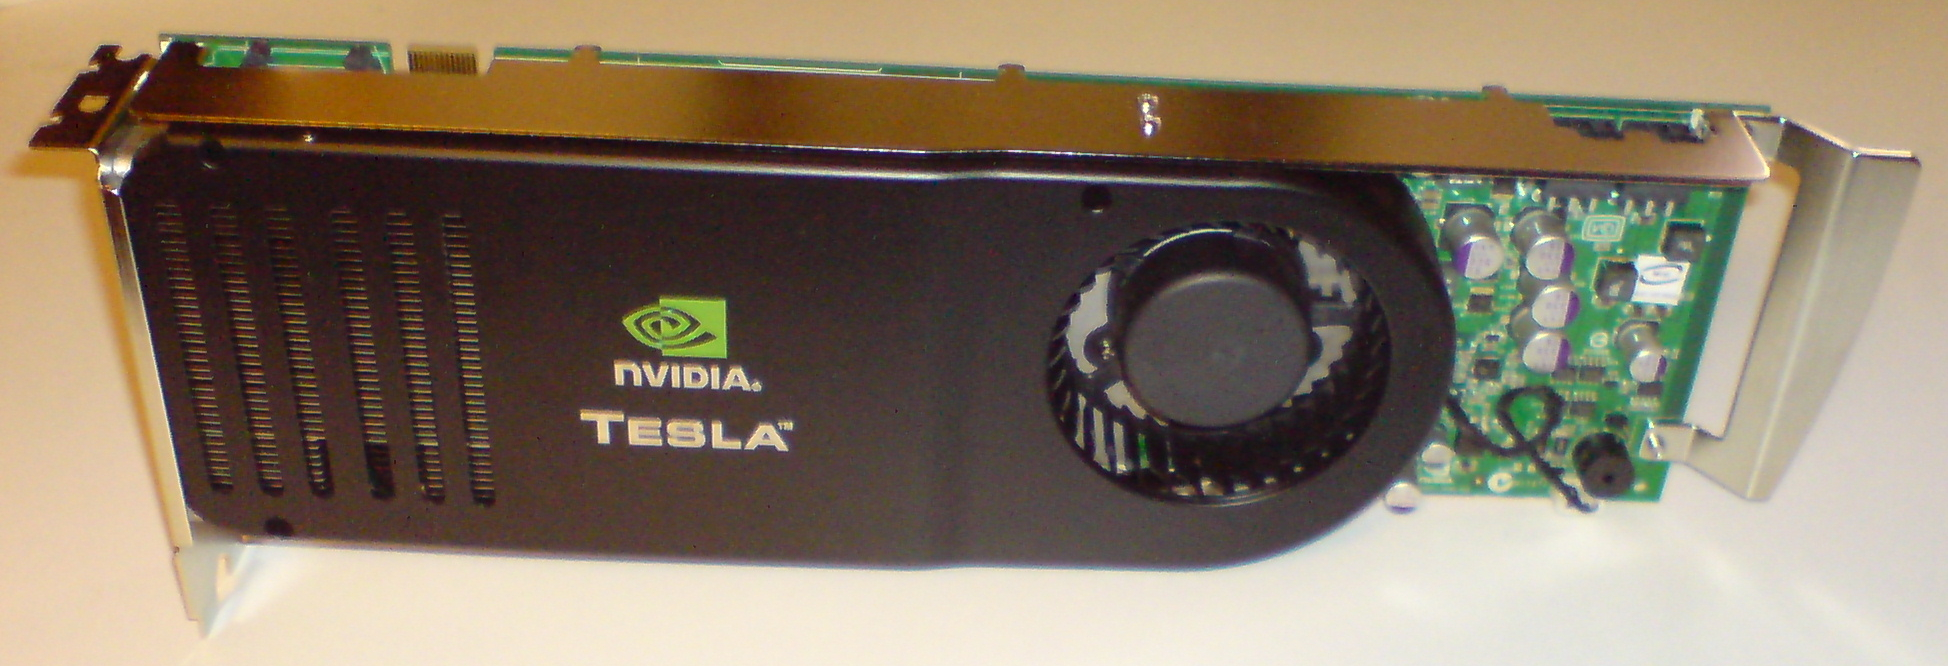
\includegraphics[width=\textwidth]{nvidiatesla.jpg}
\end{frame}

\begin{frame}
  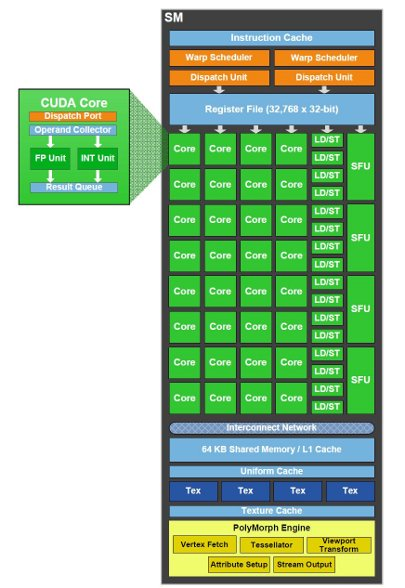
\includegraphics[height=\textheight]{gpu_sm.jpg}
\end{frame}

\end{document}